\chapter{Cluster Management}
\label{chap:cluster_management}



\section{Introduction}

A cluster is a system of computing nodes connecting to each others using some
networking infrastructure. To improve the communication among the nodes, torus
network is often used. Also, there're important things to concern when we set up
a cluster.

\begin{enumerate}
  \item All nodes must install the same OS distro (e.g. Ubuntu, or RHEL)
  using the same kernel all on machines. Name them using an organized
  convention:  cea1, cea2, cea3, \ldots

You can do this by installing everything on one machine, and the clone the disk
(Sect.\ref{sec:disk_clone}). 

  \item Now, to make it easier to configure and maintain dozens, hundreds, or
  even thousands of servers, we need to use a configuration management software.
  This enables the administrator to easily install a new component to all
  nodes at the same time (Sect.\ref{sec:package_management_software_in_cluster})
  
  \item Install NFS, NIS to centralized account managements and file system
  sharing for each account (Sect.\ref{sec:NFS}, Sect.\ref{sec:NIS_NYS_NIS+}).
  
  \item Make sure a consistent UUID and GUID across the cluster
  (Sect.\ref{sec:UUID_GUID}). 
  
  \item Synchronized clock across nodes in the cluster:
  Sect.\ref{sec:NTP}.
  
  \item Install MUNGE on all nodes for authentication: Sect.\ref{sec:MUNGE}
  
  
  \item Using modules to create a dynamic modification of user's environment
  (Sect.\ref{sec:modules}). This allows user to select a particular version of
  the package they want to use easily.
  
  \item Using a software to launch parallel task: 
  
  \begin{itemize}
    \item SLURM (Sect.\ref{sec:SLURM}): main choice for very large sites, e.g.
    Petaflop systems.
    
    
    \item Sun Grid Engine (SGE) - Sect.\ref{chap:SGE} - small and medium sites
    with an easy to deploy/integration with a complete management GUI. 
    
    
    \item TORQUE/Maui - Chap.\ref{chap:TORQUE} : main choice for grid sites that will be integrated
in large grid infrastructures 

  \end{itemize}
\end{enumerate}

Important concepts:
\begin{enumerate}
  \item Cluster: a systems of nodes
  \item Node: a single workstation
  \item Partition: a subset of the cluster, i.e. a logical set of nodes (which
  can be redundant) with the same characteristics. 
\end{enumerate}


\section{Single-system image (SSI) vs. Disk-full systems}


\url{https://help.ubuntu.com/community/AutomatedNodeDeployment}


\subsection{SSI}

This is a low-cost option for building a cluster where you install the OS and
all package in one machine, and it will mount the kernels and drivers to every
other nodes in the cluster once booted up using PXE method. Then, you can use
the computing power from these nodes, but the data is stored in one machines.

This is aka {\bf diskless shared root cluster}, and the other nodes don't need
the disk. Similar technologies are VMScluster (OpenVMS) or TruCluster (Tru64
UNIX) from Hewlett-Packard (HP).

Example:
\begin{enumerate}
  \item Kerrighed, Fig.\ref{fig:SSI_Kerrighed}
  \item OpenSSI
  \item openMOSIX
  \item LinuxPMI
  \item TrueCluster
  \item 
\end{enumerate}

\begin{figure}[hbt]
  \centerline{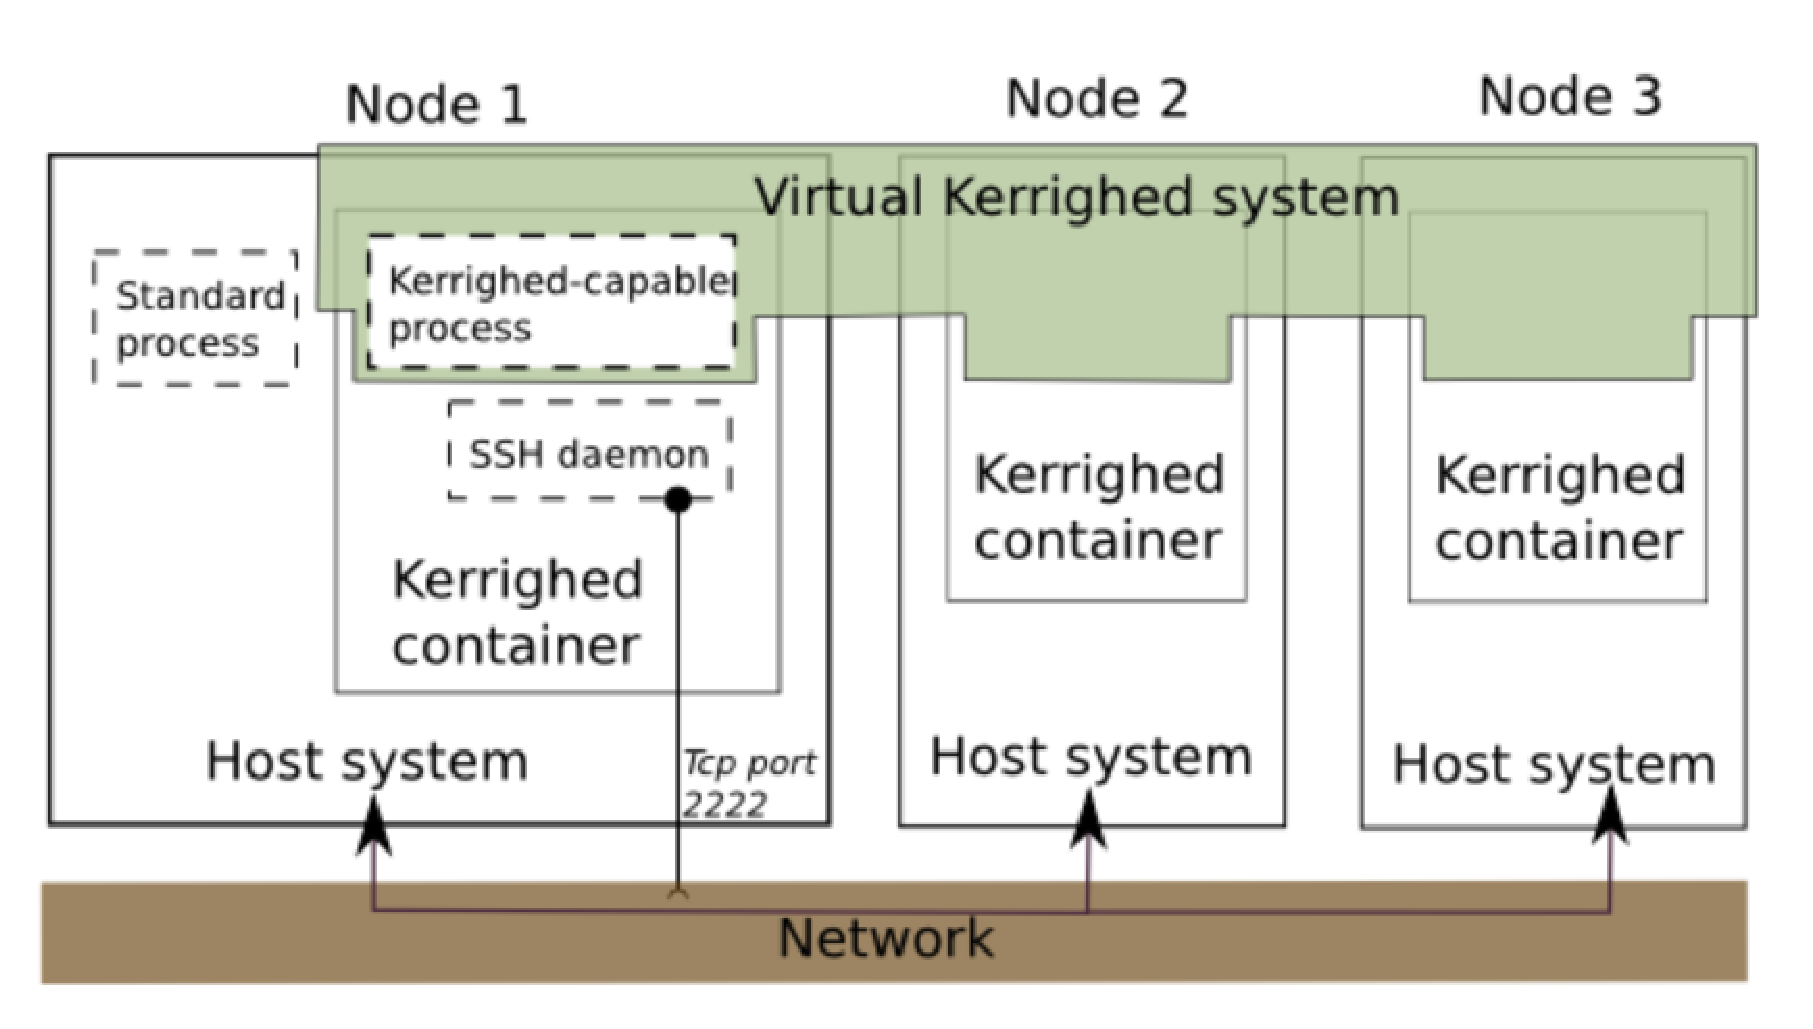
\includegraphics[height=8cm,
    angle=0]{./images/SSI_Kerrighed.eps}}
\caption{Kerrighed}
\label{fig:SSI_Kerrighed}
\end{figure}

\subsection{Disk-full systems}

Install Ubuntu 12.04 on a system that you use as the deployment server.
\begin{enumerate}
  \item Create folder to keep the scripts
\begin{verbatim}
 //bash scripts
mkdir -p /opt/cluster/
 //configuration information
mkdir -p /opt/cluster/config
\end{verbatim}

  \item Create: /opt/cluster/config/global.conf contains information about
  (1) network, (2) server ID, (3) file locations, (4) OS, (5) packages, (6) nodes.
\begin{verbatim}
# /opt/cluster/config/global.conf: configuration file for node deployment 
# This file is sourced by files used by the deployment system 

# Site information 
## identify how our cluster is configured
DOMAIN_NAME="home.local" 
DOMAIN_ADMIN="root" 
NETWORK="10.10.1.0" 
SUBNET_MASK="255.255.255.0" 
BROADCAST="10.10.1.255" 
ROUTER_NAME="router" 
ROUTER_IP="10.10.1.1" 
NAME_SERVER_NAME="dns" 
NAME_SERVER_IP="10.10.1.10" 
NTP_SERVER_NAME="ntp" 
NTP_SERVER_IP="10.10.1.10" 
DHCP_SERVER_NAME="dhcp" 
DHCP_SERVER_IP="10.10.1.10" 
HTTP_SERVER_NAME="www" 
HTTP_SERVER_IP="10.10.1.10" 
PROXY_SERVER_NAME="proxy" 
PROXY_SERVER_IP="10.10.1.10" 
TFTP_SERVER_NAME="tftp" 
TFTP_SERVER_IP="10.10.1.10" 
NFS_SERVER_NAME="nfs" 
NFS_SERVER_IP="10.10.1.10" 
MIRROR_SERVER_NAME="mirror" 
MIRROR_SERVER_IP="10.10.1.10" 

# Service information 
## identify various services and their related configuration files
DHCPD_CONFIG_FILE="/etc/dhcp3/dhcpd.conf" 
DNS_CONFIG_FILE="/etc/bind/named.conf.local" 
DNS_FORWARD_CONFIG="/etc/bind/db.$DOMAIN_NAME" 
DNS_REVERSE_CONFIG="/etc/bind/db.10.10.1" 
UBUNTU_MIRROR_URL="http://$MIRROR_SERVER_NAME.$DOMAIN_NAME/ubuntu" 
NFS_CONFIG_FILE="/etc/exports" 
NFS_ROOT_EXPORT="/srv/nfsroot" 
NFS_HOME_EXPORT="/srv/cluster" 
OFFICIAL_MIRROR="us.archive.ubuntu.com/ubuntu" 
MIRROR_LIST_FILE="/etc/apt/mirror.list" 
TFTP_ROOT="/var/lib/tftpboot" 
DEFAULT_PXE_CONFIG_FILE="$TFTP_ROOT/pxelinux.cfg/default" 

# NODE information 
## the name of the first node in the cluster
## and node information
HEAD_NODE="headnode" 
HEAD_NODE_IP="10.10.1.10" 
HEAD_NODE_WORKING_DIR="/root" 
HEAD_NODE_CONFIG_DIR="/opt/cluster/config" 
BASE_NODE_NAME="node" 
NODE_NUMBER=71 
MASTER_NODE_LIST="$HEAD_NODE_CONFIG_DIR/nodes.txt" 
NEW_NODES_LIST="$HEAD_NODE_CONFIG_DIR/new_nodes.txt" 
PSSH_HOST_FILE="$HEAD_NODE_CONFIG_DIR/hosts.txt" 
# Undiscovered node DHCP Range 
DHCP_RANGE_START="10.10.1.100" 
DHCP_RANGE_STOP="10.10.1.200" 
NODE_USER="cluster" 
NODE_USER_UID=1010 

# NFS Root filesystem information
## information related to creating NFS root for disk-less systems 
ARCH="amd64" 
RELEASE="jaunty" 
PRE_INST_PKGS="language-pack-en,language-pack-en-base,vim,wget,openssh-server,ntp,nfs-common" 
PRE_INST_EXCL_PKGS="ubuntu-minimal" # separated by a comma 
POST_INST_PKGS="linux-image-server" #separated by a space 
PKGS_TO_PURGE="" # separated by a space 
NODE_PXE="$TFTP_ROOT/nodes/$RELEASE/$ARCH" 
REPOSITORY="main restricted universe multiverse" 
NFS_BUILD_DIR="$HEAD_NODE_WORKING_DIR/nfsroot/$RELEASE/$ARCH" 
APT_SOURCES_FILE="$NFS_BUILD_DIR/etc/apt/sources.list" 
FSTAB_FILE="$NFS_BUILD_DIR/etc/fstab" 
HOSTNAME_FILE="$NFS_BUILD_DIR/etc/hostname" 
NTP_CONF_FILE="$NFS_BUILD_DIR/etc/ntp.conf" 
INTERFACE_FILE="$NFS_BUILD_DIR/etc/network/interfaces" 
HOSTS_FILE="$NFS_BUILD_DIR/etc/hosts" 
CURRENT_PXE_FILES="$HEAD_NODE_CONFIG_DIR/pxefiles.txt" 

printf "Global configration file loaded\n"
\end{verbatim}


Here is for the Lab:
\begin{verbatim}
# /opt/cluster/config/global.conf: configuration file for node deployment 
# This file is sourced by files used by the deployment system 

# Site information 
DOMAIN_NAME="jafri_lab" 
DOMAIN_ADMIN="root" 
NETWORK="10.10.1.0" 
SUBNET_MASK="255.255.255.0" 
BROADCAST="10.10.1.255" 
ROUTER_NAME="router" 
ROUTER_IP="10.10.1.1" 
NAME_SERVER_NAME="dns" 
NAME_SERVER_IP="10.10.1.10" 
NTP_SERVER_NAME="ntp" 
NTP_SERVER_IP="10.10.1.10" 
DHCP_SERVER_NAME="dhcp" 
DHCP_SERVER_IP="10.10.1.10" 
HTTP_SERVER_NAME="www" 
HTTP_SERVER_IP="10.10.1.10" 
PROXY_SERVER_NAME="proxy" 
PROXY_SERVER_IP="10.10.1.10" 
TFTP_SERVER_NAME="tftp" 
TFTP_SERVER_IP="10.10.1.10" 
NFS_SERVER_NAME="nfs" 
NFS_SERVER_IP="10.10.1.10" 
MIRROR_SERVER_NAME="mirror" 
MIRROR_SERVER_IP="10.10.1.10" 

# Service information 
DHCPD_CONFIG_FILE="/etc/dhcp3/dhcpd.conf" 
DNS_CONFIG_FILE="/etc/bind/named.conf.local" 
DNS_FORWARD_CONFIG="/etc/bind/db.$DOMAIN_NAME" 
DNS_REVERSE_CONFIG="/etc/bind/db.10.10.1" 
UBUNTU_MIRROR_URL="http://$MIRROR_SERVER_NAME.$DOMAIN_NAME/ubuntu" 
NFS_CONFIG_FILE="/etc/exports" 
NFS_ROOT_EXPORT="/srv/nfsroot" 
NFS_HOME_EXPORT="/srv/cluster" 
OFFICIAL_MIRROR="us.archive.ubuntu.com/ubuntu" 
MIRROR_LIST_FILE="/etc/apt/mirror.list" 
TFTP_ROOT="/var/lib/tftpboot" 
DEFAULT_PXE_CONFIG_FILE="$TFTP_ROOT/pxelinux.cfg/default" 

# NODE information 
HEAD_NODE="cea1" 
HEAD_NODE_IP="10.10.1.10" 
HEAD_NODE_WORKING_DIR="/root" 
HEAD_NODE_CONFIG_DIR="/opt/cluster/config" 
BASE_NODE_NAME="node" 
NODE_NUMBER=71 
MASTER_NODE_LIST="$HEAD_NODE_CONFIG_DIR/nodes.txt" 
NEW_NODES_LIST="$HEAD_NODE_CONFIG_DIR/new_nodes.txt" 
PSSH_HOST_FILE="$HEAD_NODE_CONFIG_DIR/hosts.txt" 
# Undiscovered node DHCP Range 
DHCP_RANGE_START="10.10.1.100" 
DHCP_RANGE_STOP="10.10.1.200" 
NODE_USER="cluster" 
NODE_USER_UID=1010 

# NFS Root filesystem information 
ARCH="amd64" 
RELEASE="jaunty" 
PRE_INST_PKGS="language-pack-en,language-pack-en-base,vim,wget,openssh-server,ntp,nfs-common" 
PRE_INST_EXCL_PKGS="ubuntu-minimal" # separated by a comma 
POST_INST_PKGS="linux-image-server" #separated by a space 
PKGS_TO_PURGE="" # separated by a space 
NODE_PXE="$TFTP_ROOT/nodes/$RELEASE/$ARCH" 
REPOSITORY="main restricted universe multiverse" 
NFS_BUILD_DIR="$HEAD_NODE_WORKING_DIR/nfsroot/$RELEASE/$ARCH" 
APT_SOURCES_FILE="$NFS_BUILD_DIR/etc/apt/sources.list" 
FSTAB_FILE="$NFS_BUILD_DIR/etc/fstab" 
HOSTNAME_FILE="$NFS_BUILD_DIR/etc/hostname" 
NTP_CONF_FILE="$NFS_BUILD_DIR/etc/ntp.conf" 
INTERFACE_FILE="$NFS_BUILD_DIR/etc/network/interfaces" 
HOSTS_FILE="$NFS_BUILD_DIR/etc/hosts" 
CURRENT_PXE_FILES="$HEAD_NODE_CONFIG_DIR/pxefiles.txt" 

printf "Global configration file loaded\n"
\end{verbatim}

\end{enumerate}


\section{Configuration management tool in a cluster}
\label{sec:package_management_software_in_cluster}
\label{sec:configuration-tool}
\label{sec:cluster-management-tool}

To manage a homogeneous system, and manage the installation of packages to
machines in a cluster easily, we use configuration management (CM) softwares
\footnote{\url{http://en.wikipedia.org/wiki/Comparison_of_open_source_configuration_management_software}}.

A CM tool is a robot or daemon that keeps track of files, packages, services,
and other pieces of machines in your environment, and keeping them up-to-date
for you. There are many choices, we can list some free softwares
\begin{enumerate}
  \item Puppet: 
  \item Cfengine:
  \item Chef
  \item Ansible - Sect.\ref{sec:Ansible}
  \item Salt:
  \item Bcfg2:
\end{enumerate}
All of these tools are mature and (perhaps with a little extra coding) can do
anything you need to run your environment.
\url{https://www.usenix.org/system/files/login/articles/105457-Lueninghoener.pdf}

\url{http://en.wikipedia.org/wiki/Comparison_of_open-source_configuration_management_software}

\url{http://www.infoworld.com/article/2609482/data-center/review--puppet-vs--chef-vs--ansible-vs--salt.html}

CFEngine is actually significantly older than Puppet or Chef, dating back to
1993. CFEngine has been described as the grandfather of configuration management
tools. \footnote{\url{http://www.scriptrock.com/blog/puppet-vs-cfengine}}
CFEngine runs on C, as opposed to Puppet's use of Ruby.
The learning curve of CFEngine is very steep. It does mean though that CFEngine
has a dramatically smaller memory footprint, it runs faster and has far fewer
dependencies. 

Whereas Puppet and Chef will appeal to developers and development-oriented
shops, Salt and Ansible are much more attuned to the needs of system
administrators. Puppet's model-driven approach means a smaller learning curve,
which makes it a preferred option for sysadmins with limited coding experience.
The model-driven approach also takes on a lot of the responsibility for
dependency management.

Salt is the sleekest and most robust of the four, and like Ansible it will
resonate with sys admins. Highly scalable and quite capable, Salt is hamstrung
only by the Web UI. 


Puppet is the most mature and probably the most approachable of the four from a
usability standpoint, though a solid knowledge of Ruby is highly recommended.
\textcolor{red}{Puppet is the safest bet for heterogeneous environments}, but 
you may find Ansible or Salt to be a better fit in a larger or more homogenous
infrastructure. 

\subsection{CFEngine}

\url{http://cfengine.com/product/enterprise-3-6-0/}
It's free for upto 25 machines. The price over 25-machine is not explicitly
mentioned, i.e. they adapt to the company's needs and requires contacting the
sale agents.

CFEngine has free open-source version (CFengine 2 and CFengine 3). CFEngine 3
was released in 2008 which is a  complete overhaul of its syntax and mode of
operation, and many new features such as Knowledge Management and support for
virtual environments. You specify the state in which you wish the system to be,
and CFEngine will automatically and iteratively decide the actions to take to
reach the desired state, or as close to it as possible. Underlying this ability
is a powerful theoretical model known as Promise
Theory.\footnote{\url{http://cf-learn.info/}}

CFEnterprise has 2 packages: One for Policy Server, one for Clients.
\url{http://cfengine.com/cfengine-enterprise-free-25/}

CFEngine Enterprise Vagrant Environment provides an easy way to test and explore
CFEngine Enterprise. Vagrant will create one VirtualBox VM to be the Policy
Server (server), and another machine that will be the Host Agent (client), or
host that can be managed by CFEngine.   Both will will run CentOS 6.5 64-bit and
communicate on a host-only network.
\url{https://docs.cfengine.com/latest/guide-installation-and-configuration-general-installation-installation-enterprise-vagrant.html}
\begin{itemize}
  \item Valgrant
  1.6.5:\url{http://www.vagrantup.com/download-archive/v1.6.5.html}
\end{itemize}

\subsection{Puppet}

There are two versions: Puppet (free), and Puppet Enterprise (free upto 10
nodes). \url{https://docs.puppetlabs.com/guides/platforms.html}

Puppet Labs founder and CEO Luke Kanies created the first version of Puppet in
2005 to help sysadmins easily automate common, repetitive tasks that are prone to human error. 
Puppet's language is declarative, rather than procedural. You declare the
configurations your systems need to do their jobs - for example, which versions
of operating systems they should be running - rather than prescribing the steps
that must be taken to configure them.  


The Puppet Forge is an important resource for people who use Puppet and Puppet
Enterprise. On the Forge, you'll find more than 2,700 open source modules - or
pre-written bundles of Puppet code and data - for doing a large number of common tasks

\url{http://downloads.puppetlabs.com/enterprise/sources/} 

To install Puppet:
\url{https://docs.puppetlabs.com/guides/install_puppet/install_debian_ubuntu.html}

\subsection{Chef}

There are two variants: OpenSource Chef (free) vs. Hosted Chef (free upto 25
nodes). 

\subsection{synctool}

\url{http://www.heiho.net/synctool/}


\subsection{Vagrant}
\label{sec:Vagrant}

Vagrant was originally tied to VirtualBox, but version 1.1 added support for
other virtualization software such as VMware and KVM, and for server
environments like Amazon EC2.

Vagrant is written in Ruby, but it can be used in projects written in other
programming languages such as PHP, Python, Java, \verb!C#!, and JavaScript.

Since version 1.6, Vagrant natively supports Docker containers, which in some
cases can serve as a substitute for a fully virtualized operating system.

Vagrant sits on top of virtualization software as a wrapper and helps the
developer interact easily with the providers. It automates the configuration of
virtual environments using Chef or Puppet, and the user does not have to
directly use any other virtualization software. Machine and software
requirements are written in a file called "Vagrantfile" to execute necessary
steps in order to create a development-ready box. "Box" is a format and an
extension ( .box) for Vagrant environments that is copied to another machine in
order to replicate the same environment.




\section{Modules - dynamic environment control}
\label{sec:modules}

Using \verb!Modules! package, a dynamic environment can be easily created at
different login session. In particular, depending what platform you are in
(Sect.\ref{sec:Modules-load-package-platform-dependent}) and what version of a
software/library you want to use (Sect.\ref{sec:Modules-load-package}), you can
easily select which version to use without change the PATH or MANPATH
environment variables.

\verb!Modules! was developed since early 1990s, and was mainly used at largest
computer centers. 

Popular commands: Sect.\ref{sec:Modules-modulecmd}
\begin{verbatim}
module avail                # to list all available modules you can load
module list                 # to list your currently loaded modules
module load <moduleName>    # to load moduleName into your environment
module unload <moduleName>  # to unload moduleName from your environment
module switch <oldModule> <newModule>
module display <moduleName> # display the environment variables
\end{verbatim}


\subsection{Install}
\label{sec:install-Modules}

If you don't have Modules in your system, then follow this.
If you already have Modules in your system, then read
Sect.\ref{sec:module-update-version}.

Download: there are two implementations:   
  \begin{itemize}
    \item C-version (ceased development):
    \url{http://sourceforge.net/projects/modules/files/}
    \item Tcl-version (on-going development):
    \url{http://modules.sourceforge.net/}
  \end{itemize}
The manual: modules(1) refers to C-version; and modules(4) refers to
Tcl-version.

\begin{framed}
TclX is an eXtension to Tcl, with the latest stable version is TclX8.4.1.

TclX provides new operating system interface commands, extended file control,
scanning and status commands and many others. Considered by many to be a
must-have for large Tcl apps. TclX 8.4 is installed into /usr/lib/tclx8.4.
\end{framed}
  
\subsection{-- C-version}  
  
How to install:
\url{http://nickgeoghegan.net/linux/installing-environment-modules}
\begin{enumerate}
  
  \item  The default location where it is installed is

\begin{verbatim}
BASEPREFIX = /usr/local
DEFAULTPATH = $BASEPREFIX/Modules/default
PREFIX = $BASEPREFIX$/Modules/3.2.10
EXECPREFIX = $BASEPREFIX/Modules/3.2.10
\end{verbatim}

NOTE: BASEPREFIX = \verb!/usr/local! is chosen  as it is accessible from all
users, and NFS-mounted directory built.

  \item Install to location: MODULEHOMES=/usr/local/Modules/:

{\small
\begin{verbatim}
apt-get install tcl tcl8.4-dev tclx tclx8.4-dev
tar xvvf modules-3.2.9c.tar.gz  !! <unzip the downloaded file>

cd modules-3.2.9
./configure --with-module-path=/modules 
  !! NOTE: To build with tclX (optional: to improve some operations), we add
     --with-tclx-inc=/usr/include/tclx8.4/ 
     --with-tclx-lib=/usr/lib/tclx8.4 --with-tclx-ver=8.4
  ! --with-tclx=/usr/lib : folder contain tclxConfig.sh 
  ! --with-tclx-lib=/usr/lib/tclx8.4 : folder containing LIB
  ! --with-tclx-inc=/usr/include/tclx8.4 : folder containing include files
  ! If tclxConfig.sh is not found, use the content in
  ! https://raw.githubusercontent.com/Starlink/tclx/master/unix/tclxConfig.sh.in
  
  !! NOTE: By default, installed folder is /usr/local/Modules
  !        If you want to install a different folder, use 
  !    --prefix=/path/to/new/location
  
make 
make install
\end{verbatim}
}
\url{http://sourceforge.net/p/modules/wiki/FAQ/#module-command}

   \item Finally, you need to configure .bashrc file -
   Sect.\ref{sec:.bashrc_Modules}
\end{enumerate}

\subsection{-- Tcl-version}

Both v3.2 and >=v4.0 are quite similar and transition to the new major version
should be smooth.
\url{https://modules.readthedocs.io/en/latest/MIGRATING.html}

Starting from v4.0, the Modules project provides the module command based on the
native Tcl implementation as main version instead of the traditional C version.
As a result, Modules-Tcl has become Modules. 
 

Default location:
\begin{verbatim}
/usr/local/modules-tcl
\end{verbatim}

\subsection{-- troubleshoot install}

\begin{mdframed}
On modules-3.2.10, building failes due to
\begin{verbatim}
cmdModule.c: In function 'Execute_TclFile':
cmdModule.c:643:35: error: 'Tcl_Interp' has no member named 'errorLine'
\end{verbatim}
as \verb!errorLine! is a deprecated feature in Tcl. A temporary fix is to enable
this feature
\begin{verbatim}
bash> export CPPFLAGS="-DUSE_INTERP_ERRORLINE"
bash> ./configure ... 
\end{verbatim}
\url{http://sourceforge.net/p/modules/bugs/62/}

References: read papers on \url{http://modules.sourceforge.net/}
\end{mdframed}


You may have a Tcl interpreter that causes problems with the “module” command
(which also uses Tcl). Due to this conflict, if you run any “module” commands
after loading SIMPSON, you will see the warning message
 
\begin{verbatim}
init.c(573):WARN:162: Cannot initialize TCLX modules using extended
\end{verbatim}
This warning message should not cause any problems.
\url{https://arc-ts.umich.edu/flux/software/simpson/}

\subsection{-- initialize: : module() function, load .modulespath
file and Modules's specific environment variables}
\label{sec:Modules-init}
\label{sec:.modulespath}
\label{sec:Module-environment-variables}
\label{sec:MODULEPATH}

Configure the login shell to define Modules' specific environment
variables (\verb!MODULE_VERSION!, \verb!MODULESHOME!, and \verb!MODULEPATH!),
and define the \verb!module()! alias or shell function. 

\begin{enumerate}
  \item MODULESHOME: where \verb!modulecmd! resides

Consider the \verb!MODULESHOME=/usr/local/Modules/3.2.10!.
  
  \item MODULEPATH: the path that \verb!modulecmd! searches for modulefiles
  (recurisvely), e.g. \verb!/modules!
  
We can set this path inside a module file using \verb!module use! -
Sect.\ref{sec:MODULEPATH-update}
  
  \item \verb!MODULE_VERSION!
  
  \item \verb!MODULE_VERSION_STACK!
  
  \item LOADEDMODULES		: hold the names of all loaded modules, in relative to
  the location specified in \verb!MODULEPATH!

  \item \verb!MODULEPATH!: configure the locations where to search for module
  files (Sect.\ref{sec:modulefiles}) by loading the file
  \verb!$MODULESHOME/.modulespath!

\begin{verbatim}
/usr/local/Modules/versions				# location of version files
/usr/local/Modules/$MODULE_VERSION/modulefiles	# Module pkg modulefiles (if versioning)
#/usr/local/Modules/modulefiles	# Module pkg modulefiles (if no versioning)
/modules				# General module files
\end{verbatim}
The extra-location \verb!/modules! is added during installing of Modules package
using \verb!--with-module-path! option (Sect.\ref{sec:install-Modules}).

  \item once initialized, the snapshot of the environment is saved as either (if
  BEGINENV=1) \verb!$HOME/.modulesbeginenv! or (if BEGINENV=99) whatever
  \verb!$MODULESBEGINENV! points to.

\end{enumerate}
Check more examples in module file  \verb!$MODULESHOME/modulefiles/modules! file
- Sect.\ref{sec:Modules-modules}
\footnote{\url{http://modules.sourceforge.net/man/module.html}}.

Reference: \url{http://modules.sourceforge.net/c/module.html}

There are shell-specific initialization script that has been written to do all
of that in folder \verb!$MODULESHOME/init!.  

\begin{mdframed}
NOTE: Folder structure
{\tiny
\begin{verbatim}
$MODULESHOME/bin
	where modulecmd binary is stored
	
$MODULESHOME/init
	where the settings for each shell is stored
	(a common login environment)
	.cshrc		used by csh, tcsh, 
	.profile	used by sh/zsh/ksh
	.bashrc		used by bash
	
	and an important hidden file 
$MODULESHOME/init/.modulepath
	
	
$MODULESHOME/modulefiles
	contains all modulefiles comed with Modules package
	most important: 'modules' Modulefiles
\end{verbatim}
}
\end{mdframed}

% You need to load the corresponding file in \verb!init! folder, to configure
% necessary environment variable. E.g.: in \verb!~/.bashrc! file, at the beginning
% \begin{verbatim}
% export MODULE_VERSION=3.2.10
% export MODULESHOME=/usr/local/Modules/$MODULE_VERSION/bin
% export MODULEPATH=/modules:$MODULESHOME/../modulefiles
% case "$0" in
%           -sh|sh|*/sh)	modules_shell=sh ;;
%        -ksh|ksh|*/ksh)	modules_shell=ksh ;;
%        -zsh|zsh|*/zsh)	modules_shell=zsh ;;
%     -bash|bash|*/bash)	modules_shell=bash ;;
% esac
% if [ -f $MODULESHOME/../init/$modules_shell ]; then
%     . $MODULESHOME/../init/$modules_shell
% fi
% \end{verbatim}


%The setting in \verb!~/.bashrc! file (Sect.\ref{sec:.bashrc_Modules}) helps to
%configure
The \verb!module! command alias or function which 
  
\begin{enumerate} 
  
  \item  in several shell:  it executes the
\verb!modulecmd! program (Sect.\ref{sec:Modules-modulecmd}) on the right linux
shell: which is the one we needs to use to load/unload a package of a given
version (Sect.\ref{sec:Modules-modules}).

For bash shell, it uses \verb!$MODULESHOME/../init/bash!
file, and the function is 

{\tiny
\begin{verbatim}
module() { eval `/usr/local/Modules/$MODULE_VERSION/bin/modulecmd $module_shell $*`; }
\end{verbatim}
}

  \item inside perl interpreter or Python
  GIL: it is defined as
  
\begin{verbatim}
  import os;
  if os.environ.has_key('PYTHONPATH'):
      os.environ['PYTHONPATH'] += ':/usr/local/Modules/3.2.10/init';
  else:
      os.environ['PYTHONPATH'] = '/usr/local/Modules/3.2.10/init';

  from python import module;
\end{verbatim}

\begin{verbatim}
  use lib "/usr/local/Modules/3.2.10/init";
  use perl;
\end{verbatim}

\end{enumerate}


\subsection{------ user-level}
\label{sec:.bashrc_Modules}

There are two ways to tell  loading the right file.

\begin{enumerate}
  \item automatically:

Make sure you add 
\begin{verbatim}
export MODULE_VERSION=3.2.10
\end{verbatim}
to the beginning of the \verb!~/.bashrc! - reload the file, then run:
\begin{verbatim}
/usr/local/module-3.2.10/Modules/bin/add.modules
\end{verbatim}
which add the codes (to help defining the requires environment variables) to
\verb!~/.bashrc! file.

  \item manually (recommended):

Here, you add the content of the appriate file  in
\verb!/usr/local/Modules/3.2.10/init/! to the right shell resource file.  

\begin{verbatim}
//~/.bashrc file
export MODULE_VERSION=3.2.10
export MODULESHOME=/usr/local/Modules/$MODULE_VERSION/bin
export MODULEPATH=/modules:$MODULESHOME/../modulefiles
case "$0" in
          -sh|sh|*/sh)	modules_shell=sh ;;
       -ksh|ksh|*/ksh)	modules_shell=ksh ;;
       -zsh|zsh|*/zsh)	modules_shell=zsh ;;
    -bash|bash|*/bash)	modules_shell=bash ;;
esac
if [ -f $MODULESHOME/../init/$modules_shell ]; then
    . $MODULESHOME/../init/$modules_shell
fi
\end{verbatim}
  
The above does a number of things - Sect.\ref{sec:Modules-init}). 

 \item Logout and login the shell so that \verb!module! command can be detected.
\end{enumerate}


\subsection{------ system-wide level}

If you load module files (Sect.\ref{sec:Modules-modules}), you can
skip this. 
 
% When a user login, depending on the shell type, we can specify which packages
% and which version should be automatically loaded. This can be done by first
% editing the script which tells which file to run at logon
% \begin{verbatim}
%  ! copy then edit the target file
% cp etc/global/profile.modules /etc/profile.d/modules.sh
% \end{verbatim}

First, create a symbolic link
\begin{verbatim}
//sudo ln -s /usr/local/Modules/3.2.10  /usr/local/Modules/default
cd /usr/local/Modules
sudo ln -sT 3.2.10 default
\end{verbatim}
As we can have multiple versionf of Modules, we need to define a single link,
which we can map to a different version quickly (without changing the content
of the file).

Create \verb!/etc/profile.d/module.sh! file, with the new content
\begin{verbatim}
#----------------------------------------------------------------------#
# system-wide profile.modules #
# Initialize modules for all sh-derivative shells #
#----------------------------------------------------------------------#
trap "" 1 2 3
 
MODULES=/usr/local/Modules/
 
case "$0" in
    -bash|bash|*/bash) . $MODULES/default/init/bash ;;
    -ksh|ksh|*/ksh) . $MODULES/default/init/ksh ;;
    -sh|sh|*/sh) . $MODULES/default/init/sh ;;
    *) . $MODULES/default/init/sh ;; # default for scripts
esac
 
trap - 1 2 3
\end{verbatim}



\subsection{-- modulecmd: How to load a particular version to use}
\label{sec:Modules-load-package}
\label{sec:Modules-modulecmd}

NOTE:  The first argument to \verb!modulecmd! specifies the type of shell, and
the second argument is the arguments passed to module function
(\textcolor{red}{module() automates the environment configuration depending
upon the underlying linux shell, so that user doesn't have to specify the
type of shell}).
For defining the list of modules to be loaded at shell's initialization time,
read Sect.\ref{sec:module-load-at-shell-initialization}

We can list the loaded modules
\begin{verbatim}
module list
\end{verbatim}

or list the available modules to be loaded
\begin{verbatim}
module avail
\end{verbatim}

To unload a module, we do
\begin{verbatim}
module unload gcc
\end{verbatim}


To display the string content defined in \verb!module-whatis! statement in
module file (Sect.\ref{sec:module-whatis})
\begin{verbatim}
module whatis <module-name>
\end{verbatim}
NOTE:  If no \verb!<modle-name>! modulefile is specified, all 'whatis' lines
will be shown.

To search for module based on information provided in \verb!module-whatis!,
\begin{verbatim}
module keyword 'string'
module apropos 'string'
\end{verbatim}

% The
% path to \verb!module! command needs to be set in your \verb!~/.bashrc! file
% \begin{verbatim}
% export PATH=$PATH: /usr/local/Modules/3.2.10/modulefiles/
% \end{verbatim} 

\begin{verbatim}
! check current version
gcc --version

! now load a different version
module switch gcc/4.6.2

! load the default version
module switch gcc

gcc --version
\end{verbatim}



\begin{framed}
On Blue Gene systems, all sessions must begin by loading either \verb!bgl! or
\verb!bgq! modules to designates which system one is interested in using.
\end{framed}

\textcolor{red}{Commands:}
\begin{verbatim}
 % module help

  Available Commands and Usage:

        +  add|load     modulefile [modulefile ...]
        +  rm|unload    modulefile [modulefile ...]
        +  switch       modulefile1 modulefile2
        +  display      modulefile [modulefile ...]
        +  avail|which  path [path]
        +  list
        +  help         modulefile [modulefile ...]
        
 % module help icc

----------- Module Specific Help for 'icc/7.0' --------------------

        Intel Software: Intel icc

        This module loads the lastest versions of icc.

        *** No Module Specific Help for icc/7.0 ***       
\end{verbatim}

The commands we want to use
\begin{verbatim}
module help
module list
module avail

//load
module load my_module_file
module add my_module_file
E.g.: to load the default version
module add icc
E.g.: to load a specific version
module add icc/7.0

//unload
module unload my_module_file
module rm my_module_file

//exchange one module's setting to another's
module switch my_module_file1 my_module_file2
module swap my_module_file1 my_module_file2

//show currently loaded 
module display my_module_file
module show my_module_file

//unload all
module purge

\end{verbatim}

Example: check which packages and the different versions of them
\begin{verbatim}
$module avail
------------------- /opt/packages/modules-3.2.6/modulefiles --------------------
bgl namd-bgp/2.6(default)
bgp scalasca-bgl/1.0rc2(default)
ddt-bgp/2.3-pre(default) scalasca-bgp/1.0rc2(default)
dl_poly3-bgl/3.09(default) tau-bgl
dl_poly3-bgp/3.09(default) tau-bgp
namd-bgl/2.6(default)
\end{verbatim}

We can also specify which modules to load, depending which machines you log-in.
You modify the file, depending on your shell
\begin{itemize}
  \item \verb!.cshrc.ext! (\verb!.tcshrc.ext!)
  \item \verb!.bashrc.ext!
\end{itemize}

\begin{verbatim}
if ($NERSC_HOST == "hopper") then
# Replace the following line with personal settings for Hopper
   module load fftw
endif
\end{verbatim}

\subsection{-- tclxConfig.sh}
\label{sec:tclxConfig.sh}

Content of tclxConfig.sh
{\tiny
\begin{verbatim}
##https://raw.githubusercontent.com/Starlink/tclx/master/unix/tclxConfig.sh.in

# tclxConfig.sh --
# 
# This shell script (for sh) is generated automatically by Tclx's
# configure script.  It will create shell variables for most of
# the configuration options discovered by the configure script.
# This script is intended to be included by the configure scripts
# for Tclx extensions so that they don't have to figure this all
# out for themselves.  This file does not duplicate information
# already provided by tclConfig.sh, so you may need to use that
# file in addition to this one.
#
# The information in this file is specific to a single platform.
#
# PWD: Note, just added this to keep Skycat happy.

# Tclx's version number.
TCLX_VERSION='@PACKAGE_VERSION@'

# String to pass to linker to pick up the Tclx library from its
# build directory.
TCLX_BUILD_LIB_SPEC='@TCLX_BUILD_LIB_SPEC@'

# String to pass to linker to pick up the Tclx library from its
# installed directory.
TCLX_LIB_SPEC='@TCLX_LIB_SPEC@'

# Location of the top-level source directories from which Tclx
# was built.  
TCLX_SRC_DIR='@TCLX_SRC_DIR@'
\end{verbatim}
}

Check the location \verb!/usr/local/Modules/3.2.10/!
\begin{verbatim}
$>ls /usr/local/Modules/
3.2.10  versions

$>ls /usr/local/Modules/3.2.10/
bin  init  modulefiles  share
\end{verbatim}
% Instead of using the specific location above, we assume \verb!$(MODULES)!
% represent \verb!/usr/local/Modules/3.2.10/!.

\subsection{How Modules work?}

Modules works by dynamically modify user's working environment variables based
on values stored in module files that are loaded (Sect.\ref{sec:modulefiles})
using the \verb!module! function (as defined in Sect.\ref{sec:Modules-init}).

When you run the command, for example
\begin{verbatim}
module load module-file-1
\end{verbatim}
With \verb!module-file-1! can be a file-name or a folder name. The \verb!module!
commands look for the specified name, based on some locations defined in 
\verb!$MODULESHOME/../init/.modulespath! file -
Sect.\ref{sec:.modulespath}.

\begin{enumerate}
  \item if it is a file
  
  \item if it is a directory name
  
It will load the file 
\begin{itemize}
  \item \verb!.version! module file directly in the folder

If inside this file, \verb!ModulesVersion! is set, it will use the name as the
name of the module file and try to load it- Sect.\ref{sec:.version-module-file}

  \item \verb!.modulerc! file(s) in the folder and all subfolders

before this, the global modulerc file is sourced, too


   \item if no default module file is found (from the above two steps), it will
   sort modulefile under the directory using the 'C'
   locale, and the file with the highest lexicographically sorted is loaded.  
\end{itemize}  
  
\end{enumerate}



\subsection{-- modulefiles (Modulefile, module file)}
\label{sec:modulefiles}

A module file is a file, written in Tcl that modulecmd (\verb!module()!) command 
- Sect.\ref{sec:Modules-modulecmd} - can interpret. 
Sect.\ref{sec:write-module-file} describes how to write a module file.

\begin{mdframed}
\begin{verbatim}
/usr/local/Modules/3.2.10/modulefiles
	contains all modulefiles pre-defined with Modules package
	most important: 'modules' module file
\end{verbatim}
Sect.\ref{sec:Modules-modules} explains why the file modules is important.

\end{mdframed}

Once the syntax is correct, \verb!module! read a given module file to
load the configuration needed to use that particular package version (for a
given O/S). 


\subsection{--- default module files}
\label{sec:default-modulefiles}



\subsection{-------- 3.2.10}
\label{sec:module-update-version}

This module file define the path to the particular version (here is 3.2.10) for
Module package
\begin{verbatim}
$MODULESHOME/../versions/3.2.10
\end{verbatim}

\begin{verbatim}
module load 3.2.10
module help 3.2.10
\end{verbatim}

NOTE: Suppose we install a new version of modules, in location
\verb!/usr/local/Modules/3.3/! then, we create
\begin{verbatim}
/usr/local/Modules/versions/3.3
\end{verbatim}
and copy (from \verb!versions/3.2.10! to this file) and update the information
so that we can load to use Modules 3.3 with 
\begin{verbatim}
module load 3.3
\end{verbatim}

\subsection{-------- dot}


Basically add current folder (the folder from which we run 
\begin{verbatim}
module load dot
\end{verbatim}
to the \verb!PATH! quickly.




\subsection{-------- module-git}

\begin{verbatim}
module load module-git
\end{verbatim}
this provide the command \verb!get-modules! which clone the source of current
Module software to the local machine, and then jump to that folder


\subsection{-------- module-info (2 commands: module-info, info)}

This module shows commands (\verb!module-info! and \verb!info!) that you can use
inside your module file to inspect and get information about the local system,
in choosing the right setting

\begin{verbatim}
module-info flags

info        hostname
\end{verbatim}

RESULTS:
\begin{verbatim}
+++ module-info +++++++++++++++++++++++++++++++
flags			= 32800
mode			= load
name			= module-info
specified		= module-info
shell			= bash
shelltype		= sh
version			= module-info/default
user			= advanced
trace			= 0
tracepat		= -.*
symbols			= *undef*
+++ info ++++++++++++++++++++++++++++++++++++++
hostname		= compneuro05.watson.ibm.com
level			= 1
loaded null		= 0
library			= /usr/share/tcltk/tcl8.6
nameofexecutable	=
sharedlibextension	= .so
tclversion		= 8.6
patchlevel		= 8.6.1
\end{verbatim}

\subsection{-------- modules}
\label{sec:Modules-modules}

The module file \verb!modules!, stored in 
\begin{verbatim}
/usr/local/Modules/$MODULE_VERSION/modulefiles/modules
\end{verbatim}
is an important Modulefile (Sect.\ref{sec:modulefiles})
that everyone in any platform (Linux, Unix, \ldots) need to load.

\begin{mdframed}
By default, the modulefiles will be stored in \verb!$(MODULEHOMES)/modulefiles!.
In some OS where the package is installed by default, the location is
\begin{verbatim}
/etc/modulefiles # CentOS, Scientific Linux, RHEL
\end{verbatim}
\end{mdframed}

We need to modify this file to configure the below environment variables, using
Modules' \verb!uname! command
\begin{verbatim}
setenv MODULES_MACH [uname machine]          
setenv MODULES_OS   [uname sysname] 
setenv MODULES_OS_REL  [uname release]
setenv MODULES_OS_VER  [uname version]
setenv MODULES_HOST   [uname nodename]
setenv MODULES_DOMAIN  [uname domain] 
\end{verbatim}
and then insert 
\begin{verbatim}
module load modules
\end{verbatim}
at the beginning of user's login shell script, e.g. \verb!~/.bashrc!.
It is also a good idea to add a \verb!prereq modules! line to 
each of your modulefiles that uses these variables
(Sect.\ref{sec:Modules-prereq}).


NOTE: \verb!uname! accepts
\begin{verbatim}
    sysname - the operating system name 
    nodename - the hostname 
    domain - the name of the domain 
    release - the operating system release 
    version - the operating system version 
    machine - a standard name that identifies the system's hardware 
\end{verbatim}
\url{http://modules.sourceforge.net/man/modulefile.html#lbAD}


To test, in shell prompt
\begin{verbatim}
printenv | grep MODULES
\end{verbatim}

\subsection{-------- null}

This is the simplest module file (that you can copy and start with), it does
nothing.

\subsection{-------- use.own}

This module file, create a folder name \verb!$HOME/privatemodules!, and append
to the \verb!MODULEPATH!, so that you can define your own module files in that
location. 

\begin{verbatim}
module load use.own
\end{verbatim}

REMEMBER: Load this before you load any module files defined in
\verb!$HOME/privatemodules! folder.

\subsection{--- create your own module file}

\begin{mdframed}

{\bf How it works}: A list of modulefiles, each defined for a particular version
of a package, is saved in a location that can be searched. The default
modulefiles searchpath is specified in a hidden configuration file -
Sect.\ref{sec:.bashrc_Modules}
\begin{verbatim}
/usr/local/Modules/3.2.9/init/.modulespath
\end{verbatim}

\end{mdframed}

\subsection{------- step 1: choose location}

You can have your set of modulefiles that can be organized into these folders
\begin{itemize}
  \item Choice 1:
  
\begin{verbatim}
Put all in to this folder
/modules/

and packages are into this
/packages/

\end{verbatim}
or (for user-specific setting) we can put \verb!~/packages, ~/modules! folders.

The location \verb!/modules! folder need to be configured: either at the time of
install Modules (which was done by using --with-module-path option when
compiling), or manually by either configure the environment variable MODULEPATH
or modify the file
\begin{verbatim}
 ! edit the file
 ! comment out all; except the line with /modules
vim /usr/local/Modules/3.2.9/init/.modulespath
\end{verbatim}

Also, we make two important folders
\begin{verbatim}
 ! make the folders
mkdir /packages ; mkdir /modules
\end{verbatim}

  \item Choice 2

\begin{verbatim}
Put all in to the default folder
/usr/local/Modules/3.2.10/modulefiles

\end{verbatim}
\end{itemize}
User need to know the information of a package, as given in MODULEPATH, which
include tool name and version number in order to load the package
(Sect.\ref{sec:Modules-load-package}).

\subsection{------- step 2: write your module file}
\label{sec:write-module-file}

A modulefiles is a script file written in Tcl language, starting with a magic
code \verb!#%Module! (a version number may come after, indicating the format
version of the module file). Without the version, 
\verb!modulecmd! will assume the modulefile is compatible with the latest
version. The current latest version is 1.0.

Check all
commands we can
use: \footnote{\url{http://modules.sourceforge.net/c/modulefile.html}}

\textcolor{red}{Examples can be learnt from default module files}
(Sect.\ref{sec:default-modulefiles}).

For each version of a particular package, we needs a dedicated Modulefile,
typically stored in the one of the locations as defined by \verb!MODULEPATH!
environment variable. Example: 
\begin{verbatim}
export MODULEPATH=/modules

/modules/gcc/4.7   file for GCC 4.7.x
/modules/gcc/5.2   file for GCC 5.2.x
\end{verbatim}

\begin{mdframed}
Guidelines:
\begin{verbatim}
	e.g. 
	$MODULEPATH/tools/tool_name/version_number

and packages into these different folder
/tools/
	contain code for other software tools
	e.g.: /tools/vendor_name/tool_name/version_number
	
/groups/
	contain code for various teams (designers, verification, FPGA)
	e.g.: 
/projects/
	contain code for design projects

\end{verbatim}
\end{mdframed}


Le'ts look at the content of a Modulefile. A typical modulefile is a simple bit
of code that set or add entries to the PATH, MANPATH, or other environment
variables; and provide information that get return when we call
\begin{verbatim}
module help <module-name>
module whatis <module-name>
\end{verbatim}

In this file, we put every evironment variables we need to configure for that
package version.
\url{http://modules.sourceforge.net/man/modulefile.html}
\url{https://fs.hlrs.de/projects/craydoc/docs/books/S-2393-31/html-S-2393-31/appendix-5ptgipw3-las-creatingmodulefiles.html}
\url{https://wiki.scinet.utoronto.ca/wiki/index.php/Installing_your_own_modules}
\url{https://wiki.scinet.utoronto.ca/wiki/index.php/Brian}

\textcolor{red}{\bf IMPORTANT: Use absolute directory, don't use tilde
} (\verb!~!) in your path; otherwise, module doesn't know how to unset the
path.

Example: a \verb!/modules/intel-mkl/10.1.0.015!
file's content
\begin{verbatim}
#%Module1.0
proc ModulesHelp { } {
 global dotversion
 puts stderr "\tIntel MKL 10.1.0.015"
}
module-whatis "Intel MKL 10.1.0.015"
conflict intel-mkl
setenv MKLROOT /ichec/packages/intel/mkl/10.1.0.015
prepend-path INCLUDE /ichec/packages/intel/mkl/10.1.0.015/include
prepend-path LD_LIBRARY_PATH /ichec/packages/intel/mkl/10.1.0.015/lib/em64t
prepend-path MANPATH /ichec/packages/intel/mkl/10.1.0.015/man
prepend-path LIBRARY_PATH /ichec/packages/intel/mkl/10.1.0.015/lib/em64t
prepend-path CPATH /ichec/packages/intel/mkl/10.1.0.015/include
prepend-path FPATH /ichec/packages/intel/mkl/10.1.0.015/include
prepend-path NLSPATH /ichec/packages/intel/mkl/10.1.0.015/lib/em64t/locale/%l_%t/%N
setenv MKL_NUM_THREADS 1
\end{verbatim}

Example: the code for \verb!/modules/gcc/4.6.2! file
\begin{verbatim}
#%Module1.0
proc ModulesHelp { } {
global dotversion
 
puts stderr "\tGCC 4.6.2 (gcc, g++, gfortran)"
}
 
module-whatis "GCC 4.6.2 (gcc, g++, gfortran)"
conflict gcc
prepend-path PATH /packages/gcc/4.6.2/bin
prepend-path LD_LIBRARY_PATH /packages/gcc/4.6.2/lib64
prepend-path LIBRARY_PATH /packages/gcc/4.6.2/lib64
prepend-path MANPATH /packages/gcc/4.6.2/man
# in GCC 4.8+
#prepend-path MANPATH /packages/gcc/4.8.0/share/man                       
prepend-path INFOPATH /packages/gcc/4.8.0/share/info
prepend-path PYTHONPATH /packages/gcc/4.8.0/share/gcc-4.8.0/python
       
setenv CC gcc
setenv CXX g++
setenv FC gfortran
setenv F77 gfortran
setenv F90 gfortran
\end{verbatim}

Example: the content for \verb!~/modules/cuda/4.2! file
NOTE: To use shell environment, we use \verb!$env(VAR_NAME)! 

\begin{verbatim}
#%Module1.0
proc ModulesHelp { } {
 global dotversion
 puts stderr "\tCUDA 4.2"
}
module-whatis "CUDA 4.2"
conflict cuda
setenv CUDA_ROOT /packages/cuda/4.2
prepend-path PATH $env(CUDA_ROOT)/cudaprof/bin
prepend-path PATH $env(CUDA_ROOT)/bin
prepend-path LD_LIBRARY_PATH $env(CUDA_ROOT)/lib64
prepend-path CPATH $env(CUDA_ROOT)/C/common/inc
prepend-path INCLUDE $env(CUDA_ROOT)/C/common/inc
setenv CUDA_NIC_INTEROP 1
\end{verbatim}

\subsection{Commands to use inside module files}

\subsection{----- commands specific to Tcl: proc, set, module-whatis}
\label{sec:module-whatis}
\label{sec:proc-Modules}
\label{sec:set-Modules}

define a function
\begin{verbatim}
proc  <ProcName> { }  {
  global  gccversion   //use variable defined outside the function

  puts stderr "string $gccversion"
}

set  gccversion   4.7.0   //define a variable to be used inside the script
\end{verbatim}

define variable (to be used inside the script)
\begin{verbatim}
set  gccversion   4.7.0   //define a variable to be used inside the script
\end{verbatim}

define string to be printed out when \verb!module whatis <module-name>! is used
\begin{verbatim}
module-whatis   "the string"
\end{verbatim}

to use the value of the variable inside the string, add \verb!$! in front
\begin{verbatim}
"my string $gccversion"
\end{verbatim}
also, to add new line (\verb!\n!), and tab (\verb!\t!) to the string.

to use the value of the variable (say \verb!gccversion!) outside the string,
enclose the name with \verb!${gccversion}!.


\subsection{----- avoid loading the same packages of different version:
conflict}

In two or more module files (each links to a different version of the same
package), suppose the package is name as 'gcc' (any name you want), then add the
line
\begin{verbatim}
conflict gcc
\end{verbatim}

Then, once a version of that package is loaded, and you load another version,
Modules will detect.

\subsection{----- read environment variable: \$env}


We use \verb!$env()! function

\begin{verbatim}
setenv GCCVERSION 4.7.0
prepend-path PATH /packages/gcc/$env(GCCVERSION)/bin
\end{verbatim}



\subsection{----- common enviroment variables to be updated (once a module is
loaded): prepend-path, setenv}

Use \verb!prepend-path! or \verb!setenv! 

\begin{verbatim}
set gccversion 4.7.0
prepend-path PATH /packages/gcc/${gccversion}/bin
prepend-path LIBDIR /packages/gcc/${gccversion}/lib64
prepend-path LD_LIBRARY_PATH /packages/gcc/${gccversion}/lib64
prepend-path LIBRARY_PATH /packages/gcc/${gccversion}/lib
prepend-path INCLUDE /packages/gcc/${gccversion}/include
prepend-path CPATH /packages/gcc/${gccversion}/include
prepend-path MANPATH /packages/gcc/${gccversion}/share/man
prepend-path INFOPATH /packages/gcc/${gccversion}/share/info
prepend-path PYTHONPATH /packages/gcc/${gccversion}/share/gcc-${gccversion}/python
\end{verbatim}


\begin{verbatim}
setenv MODULES_MACH [uname machine]
setenv MODULES_OS   [uname sysname]
setenv MODULES_OS_REL  [uname release]
setenv MODULES_OS_VER  [uname version]
setenv MODULES_HOST  [uname nodename]
setenv MODULES_DOMAIN  [uname domain]
\end{verbatim}

\subsection{------ update MODULEPATH: module use}
\label{sec:MODULEPATH-update}

\begin{verbatim}
module use   /usr/local/Modules/versions
\end{verbatim}

Check more at Sect.\ref{sec:Module-environment-variables}



\subsection{How to load modules at shell login}
\label{sec:module-load-at-shell-initialization}

Default loaded module files can be specified in some resource rc files which
contain global, user and modulefile specific setup.
\begin{enumerate}
  \item Global RC file: 
   \verb!${prefix}/etc/${MODULERCFILE}!. If \verb!${MODULERCFILE}! is not
   defined then the global RC file is assumed to be "modulerc"
  
  \item User-specific RC file: \verb!${HOME}/.modulerc!
  
  
  \item all \verb!.modulerc! and \verb!.version! files
  (Sect.\ref{sec:.version-module-file}) found during modulefile seeking in
  locations defined in Sect.\ref{sec:MODULEPATH}.
\end{enumerate}
Besides, you can also do one of the following choices

Option 1: create \verb!bash_module! file, 
\begin{verbatim}
module purge
module load module-1
module load module-2
//...
\end{verbatim}
and load this file from
\verb!~/.bashrc!
\begin{verbatim}
if [ -f ~/.bash_modules ]; then
   . ~/.bash_modules 
fi
\end{verbatim}

\textcolor{red}{Option 0}: run this command (list all modules to be loaded at
shell's initialization)
\begin{verbatim}
module initlist
\end{verbatim}

\textcolor{red}{Option 0.b}: run this command (remove all modules to be loaded
at shell's initialization)
\begin{verbatim}
module initclear
\end{verbatim}


\textcolor{red}{Option 2}: run this command (append to the existing list)
\begin{verbatim}
module initadd  module-1  module-2 
\end{verbatim}
which  add the given module files to the shell's initialization file in the
user's home directory; the shell's initialization files are those
given below (depending upon the shell)
\begin{verbatim}
csh - .modules, .cshrc(.ext), .csh_variables, and .login(.ext) 

tcsh - .modules, .tcshrc, .cshrc(.ext), .csh_variables, and .login(.ext) 

sh and ksh - .modules, .profile(.ext), and .kshenv(.ext) 

bash - .modules, .bash_profile, .bash_login, .profile(.ext), and .bashrc(.ext) 

zsh - .modules, .zcshrc(.ext), .zshenv(.ext), and .zlogin(.ext)
\end{verbatim}
If a '\verb!module load!' line is found in any of these files, the modulefile(s)
is(are) appended to any existing list of modulefiles.  If the 'module load'
line is found in multiple shell initialization files, all of the lines are changed.

\textcolor{red}{Option 3}: run this command (prepend to the beginning)
\begin{verbatim}
module initprepend module-1  module-2 
\end{verbatim}

\textcolor{red}{Option 4}: run this command (remove certain module files from
the list)
\begin{verbatim}
module initrm module-1  module-2 
\end{verbatim}

\textcolor{red}{Option 5}: run this command (switch one module file (in the
initialization list) to a different one)
\begin{verbatim}
module initswitch module-old  module-new
\end{verbatim}

\subsection{How to add a new version of the package to be controlled}

\begin{mdframed}

Now, suppose you want to have different version of CUDA, e.g. 4.2 and 5.0, or
different versions of gcc compilers. Download the source-codes and compile,
install to
\begin{verbatim}
/packages/cuda/4.2

/packages/cuda/5.0
\end{verbatim}

IMPORTANT
LINK:
\url{http://sourceforge.net/p/modules/wiki/FAQ/#i-put-the-module-command-in-a-script-and-i-run-the-script-it-doesnt-change-my-environment}
\end{mdframed}

NOTE: \textcolor{red}{It's recommended to use the lower-case for the packages
name}. What to do for each version
\begin{enumerate}
  \item Create the target folder
\begin{verbatim}
mkdir /packages/cuda/4.2 -p

  ! this is for gcc
mkdir /packages/gcc/4.6.2 -p
\end{verbatim}
 \item Download the sour-code, e.g. look into the 'Download Source Package' for
 gcc 4.3 in the right column
 \url{http://packages.ubuntu.com/lucid/gcc-4.3}
\begin{verbatim}
apt-get install lzma
unlzma gcc-4.3.4.tar.lzma
tar -xvf gcc-4.3.4.tar

\end{verbatim}


  \item Then from the source code run ./configure so that it install the output
  to this location
\begin{verbatim}
./configure --prefix=/packages/cuda/4.2

 ! this is gcc
./configure --prefix=/packages/gcc/4.6.2
\end{verbatim}
For instruction how to build gcc, check Sect.\ref{sec:gcc}.

  \item Instal the package normally
\begin{verbatim}
make -j4
make install
\end{verbatim}
\end{enumerate}

Now, we need to tell how to load a particular version of CUDA or gcc. 
\begin{verbatim}
mkdir /modules/cuda

mkdir /modules/gcc
\end{verbatim}
and edit the file
\begin{verbatim}
vim /modules/cuda/4.2

vim /modules/gcc/4.6.2
\end{verbatim}
The content of this file is copied from the template file \verb!modulefiles!
(Sect.\ref{sec:modulefiles}).

\subsection{-- configure package dependencies}
\label{sec:Modules-prereq}

Suppose if you want to load gcc/5.4.0, you need to have \verb!isl! package
loaded first. In the Modulefile (Sect.\ref{sec:modulefiles}) 
\begin{verbatim}
/modules/gcc/5.4.0
\end{verbatim}
add this line
\begin{verbatim}
prereq isl   # which only gives error if isl is not loaded

module load isl   # use this ensure it is loaded

# before
conflict gcc
\end{verbatim}

NOTE: Every modulefiles should have the dependency on modules Modulefile
(Sect.\ref{sec:Modules-modules})
\begin{verbatim}
prereq modules
\end{verbatim}

Example: make sure 'isl' package is loaded before gcc 5.4 is loaded; and only
load if it is loading gcc
\begin{verbatim}

module-whatis "GCC 5.4.0"

if { [module-info mode load ] } {
  if { [ is-loaded isl ] {
     puts stderr "The module isl is loaded"
  } else {
    module load isl
  }
}
prereq isl
conflict gcc 

// other parts for GCC next
\end{verbatim}

\subsection{-- configure platform-dependent package?}
\label{sec:Modules-load-package-platform-dependent}

From the user level, there is no need to specify the platform information when
loading a package. However, Modulefile for that package needs to know
to configure paths properly  

First, make sure you have modules Modulefile (Sect.\ref{sec:Modules-modules}) is
loaded which has information that can be used to detect current O/S or platform.
Then, in the Modulefile for your package, you use \verb!switch! statement.

Example: modulefile for tdc-shell with paths configured differently depending
the current platform of the machine user is using

\begin{verbatim}
proc ModulesHelp{}{
puts stderr "\tdc_shell - loads the environment for dc_shell\n"
}

module-whatis   "loads the environment for dc_shell"

setenv SYNOPSYS /tools/synopsys/dc/2000.11

switch -exact $env(MODULES_OS) {
  SunOS {
    set plat "sparcOS5"
  }
  HPUX {
    set plat "hpux10"
  }
  default {
     puts stderr "Error: Platform for OS $env(MACHINE_OS) not supported"
     exit
  }
}

prepend-path    LD_LIBRARY_PATH     $env(SYNOPSYS)/$plat/dcm
prepend-path    PATH                $env(SYNOPSYS)/$plat/syn/bin
set-alias syn_help "acroread /tools/synopsys/sold/2000.11/top.pdf"
\end{verbatim}

\subsection{How to set the default version for one package}
\label{sec:.version-module-file}

As we may have different versions to use, we can set a default version. Suppose
\begin{verbatim}
vim /modules/cuda/.version

vim /modules/gcc/.version
\end{verbatim}

The content of these files tell basically define \verb!ModulesVersion! with the
module file name as the default version for the package to be loaded
\begin{verbatim}
#%Module1.0
set ModulesVersion "4.6.2"
\end{verbatim}

\subsection{How to check what is configured with a package}

To see what is configured with a particular version of a package, we call
\begin{verbatim}
> module show cuda


-------------------------------------------------------------------
/modules/cuda/4.2:

module-whatis    CUDA 4.2 
conflict         cuda 
setenv           CUDA_ROOT /packages/cuda/4.2 
prepend-path     PATH /packages/cuda/4.2/cudaprof/bin 
prepend-path     PATH /packages/cuda/4.2/bin 
prepend-path     LD_LIBRARY_PATH /packages/cuda/4.2/lib64 
prepend-path     CPATH /packages/cuda/4.2/C/common/inc 
prepend-path     INCLUDE /packages/cuda/4.2/C/common/inc 
setenv           CUDA_NIC_INTEROP 1 
-------------------------------------------------------------------
\end{verbatim}

\subsection{How to set automatic initialization at shell login}


Now, to load which module for a local user, that user can put into their
\verb!~/.bashrc! file one or more \verb!module! commands
\begin{verbatim}
module purge
module load cuda/5.5
\end{verbatim}

If you have different clusters, and you want to load different modules depending
on which cluster you're logging on, then you can use an global environment
variable that tell the cluster name, e.g. \verb!$CLUSTER!. Then, in the
\verb!~/.bashrc! file. A simple approach
\begin{verbatim}
#to load gromacs only on saw: 
if [ $CLU == 'saw' ]; then module load gromacs; fi 
#to load octave on any system except saw: 
if [ $CLU != 'saw' ]; then module load octave; fi
\end{verbatim}

or a more complicated one
\begin{verbatim}
case $CLUSTER in
  orca)
  #load intel v11.1.069 when on orca instead of the default
  	module unload intel
  	module load intel/11.1.069 
  ;;
  mako)
  #alias vim to vi on mako, as the former isn't installed
    alias vim=vi
  ;;
  *)
    #Anything we want to end up in "other" here....
  ;;
esac
\end{verbatim}
\url{https://www.sharcnet.ca/help/index.php/Knowledge_Base\#How_do_I_load_different_modules_on_different_clusters.3F}


References:
\begin{enumerate}
  \item \url{http://modules.sourceforge.net/}
  
  \item
  \url{http://www.uvacse.virginia.edu/itc-clusters/the-modules-approach-to-environment-management/}
  
  \item
  \url{https://www.sharcnet.ca/help/index.php/Configuring_your_software_environment_with_Modules}
\end{enumerate}

\section{OpenSSL}
\label{sec:OpenSSL}

When you choose OpenSSL for credential authentication in a partition, this is
what will be configured in the \verb!slurm.conf! file.
\begin{verbatim}
CryptoType=crypto/openssl
JobCredentialPrivateKey = /usr/local/etc/slurm.key
JobCredentialPublicCertificate = /usr/local/etc/slurm.cert
\end{verbatim}

We first need to create the keys
\begin{verbatim}
sudo openssl genrsa -out /usr/local/etc/slurm.key 1024

sudo openssl rsa -in /usr/local/etc/slurm.key -pubout -out
               /usr/local/etc/slurm.cert
\end{verbatim}

\section{MUNGE}
\label{sec:MUNGE}

MUNGE (MUNGE Uid 'N' and Gid Emporium) is an authentication service that creates
and validates user credentials on the server, developed by LLNL. MUNGE is
designed to work in large environments such as HPC clusters. MUNGE can be used with different batch
scheduler: TORQUE/PBS or SLURM. 

Why MUNGE?
\begin{enumerate}
  \item Compared to {\it privileged port/ruserok}, MUNGE is more scalable, can
  bypass \verb!rsh! type functional call by ruserok.
  \item  authd: \url{http://www.theether.org/authd/}
\end{enumerate}

What MUNGE does? it create a security realm that encompasses a group of hosts
having common users and groups. Credentials are valid only within the security
realm. The daemons must run on every host in the realm. On each machine, you can
either download the source code and compile
\footnote{\url{https://code.google.com/p/munge/wiki/InstallationGuide}} or
install the binary package from Ubuntu.
\begin{verbatim}
apt-get install munge libmunge2 -y
\end{verbatim}
After you install, a new user (munge) and group (munge) is created, see
/etc/passwd and /etc/group. Make sure the UID and GID is unique so that it can
be shared among the hosts in the group.
\begin{verbatim}
munge:x:3000:130::/home/munge:/bin/false
\end{verbatim}
This non-root user will be used to run munge daemon. Thus, we should put them in
the NIS and update the NIS server. Notice the UID=3000 and GID=130, we need to
use them later.

\begin{mdframed}
Ubuntu 12.04 use munge 0.5.10.
\end{mdframed}

MUNGE has two utilities: \verb!munge! and \verb!unmunge!. The \verb!munge!
daemon must run on the server and all submission hosts. On most platforms,
running \verb!munge! daemon doesn't require root privileges. \verb!munged!
daemon uses the following folders
\begin{verbatim}
/etc/munge/   ; contain the daemon's secret key
/var/lib/munge/ ; contain the daemon's PRNG seed file
/var/log/munge/ ; daemon's log file
/var/run/munge/ ; contains (1) daemons's PID file, (2) Unix domain sockets for
clients to communicate with the daemon
\end{verbatim}
These folder must have appropriate privileges for the non-root user to run the
\verb!munge! daemon. Here the non-root user is \verb!munge!; we need to adjust
the permission by.
\begin{verbatim}
chmod 0700 /etc/munge
chmod 0711 /var/lib/munge
chmod 0700 /var/log/munge
chmod 0755 /var/run/munge
chown -R munge:munge /etc/munge
chown -R munge:munge /var/lib/munge
chown -R munge:munge /var/log/munge
chown -R munge:munge /var/run/munge
\end{verbatim}

% By default, /etc/munge folder contains the secret key (with recommened
% permission is 0700), /var/lib/munge to contain the PRNG seed file (permission is
% 0711), /var/log/munge to contain the log file (permission 0700), /var/run/munge
% to contain Unix domain socket for clients to communicate with the daemon
% (permission 0755).

To define a security realm, all \verb!munged! daemon on the hosts in that
group must have the same \verb!/etc/munge/munge.key! (permission 0400). To
create the secret key, use ONE of the
following methods \footnote{\burl{https://code.google.com/p/munge/wiki/InstallationGuide}}
\begin{verbatim}
// existing script (which can choose between /dev/random or /dev/urandom)
/usr/sbin/create-munge-key

// Explicit commands
;; for paranoid
dd if=/dev/random bs=1 count=1024 >/etc/munge/munge.key

;; or (for impatient)
dd if=/dev/urandom bs=1 count=1024 >/etc/munge/munge.key

;; or (using hash of a password)
echo -n "foo" | sha1sum | cut -d' ' -f1 >/etc/munge/munge.key

;; or (simple, unsecure: enter password directly) 
echo "some_password"  >  /etc/munge/munge.key
\end{verbatim}
This file should have permmission 0400 and owned by the non-privileged user that
run \verb!munged! daemon.
\begin{verbatim}
chmod 0400 /etc/munge/munge.key
chown munge:munge /etc/munge/munge.key
\end{verbatim}
Then, \textcolor{red}{Securely you copy this file
(/etc/munge/munge.key) to all hosts within the same security realm using scp}
(e.g. all mechines in the cluster).

Now, set \verb!munge! daemon to automatically run at system bootup
\begin{verbatim}
pdsh -R ssh -w cea[2-16] "update-rc.d munge defaults"
pdsh -R ssh -w cea[2-16] "/etc/init.d/munge start"
\end{verbatim}
The daemon can run using either (1) \verb!/usr/sbin/munged! or (2)
\verb!/etc/init.d/munge restart!.

The init script \verb!/etc/init.d/munge! uses the sources from
/etc/default/munge (on Debian-based system) or /etc/sysconfig/munge (on
RedHat-based system), if present, to set variables recorgnized by the script.
\begin{verbatim}
##
# Pass additional command-line options to the daemon.
##
## Use this until munge 0.5.8
# OPTIONS="--force --key-file /etc/munge/munged.key --num-threads 1"
## Use this from Munge 0.5.9
# DAEMON_ARGS="--key-file /etc/munge/munge.key --num-threads 1"

##
# Adjust the scheduling priority of the daemon.
##
# NICE=

##
# Execute the daemon under another username.
## 'munge' user is used by default 
# USER="munge"
\end{verbatim}
\url{https://code.google.com/p/munge/source/browse/src/etc/munge.sysconfig?name=munge-0.5.9}

Finally, to test the installation
\begin{verbatim}
   // generate a credential to stdout
minhtuan@cea1:$HOME\ $munge -n
MUNGE:AwQDAAAZ/EcVcsoYXrHTgF45XXXUPbBuK+NMUuWsrMRG9XP9jZZBH63BYupL1c+RlCoOuHM2o0eX9WGeWK/YmaYj9XHwfmSIfMwTuOOxmhz2S5GyWHtCeXY=:

  // Check if the generated credential can be locally decoded with 'unmunge'
minhtuan@cea1:$HOME\ $munge -n | unmunge
STATUS:           Success (0)
ENCODE_HOST:      cea1.gmu.edu (199.26.254.42)
ENCODE_TIME:      2012-09-06 06:25:36 (1346927136)
DECODE_TIME:      2012-09-06 06:25:36 (1346927136)
TTL:              300
CIPHER:           aes128 (4)
MAC:              sha1 (3)
ZIP:              none (0)
UID:              minhtuan (2016)
GID:              users (100)
LENGTH:           0

  // Check if the generated credential can be decoded from a remote machine in
  // the group
minhtuan@cea1:$HOME\ $munge -n | ssh cea2 unmunge
STATUS:           Success (0)
ENCODE_HOST:      cea1.gmu.edu (199.26.254.42)
ENCODE_TIME:      2012-09-06 06:25:50 (1346927150)
DECODE_TIME:      2012-09-06 06:29:34 (1346927374)
TTL:              300
CIPHER:           aes128 (4)
MAC:              sha1 (3)
ZIP:              none (0)
UID:              minhtuan (2016)
GID:              users (100)
LENGTH:           0

  // Quick benchmark
minhtuan@cea1:$HOME\ $remunge
2012-09-06 06:26:00 Spawning 1 thread for encoding
2012-09-06 06:26:00 Processing credentials for 1 second
2012-09-06 06:26:01 Processed 7765 credentials in 1.001s (7758 creds/sec)
\end{verbatim}

You can use the interface provided in \verb!<munge.h>! header file, which
require installing.
\begin{verbatim}
apt-get install libmunge-dev 
\end{verbatim}

\subsection{MUNGE - TORQUE}
\label{sec:MUNGE_TORQUE}

Other options for authentication in TORQUE to authorize client applications:
privileged port/ruserok.

MUNGE is supported from TORQUE 2.5.3.
\footnote{\url{http://www.clusterresources.com/pipermail/torquedev/2010-October/002989.html}}
\url{http://www.filewatcher.com/p/torque-2.5.4-1.el6.x86_64.rpm.49736/usr/share/doc/torque-2.5.4/Release_Notes.html}

We can use only one authentication method at a time. With TORQUE, we need to
choose from compile time, i.e. compile TORQUE with MUNGE enabled
\begin{verbatim}
./configure -enable-munge-auth
\end{verbatim}

TORQUE doesn't link any part of the MUNGE library into its executables. Instead,
it calles \verb!munge! or \verb!unmunge!. TORQUE client utilities call
\verb!munge! and then deliver an encrypted credential to \verb!pbs_server!
where the credential is uncrypted (\verb!unumnged!) and the server verifies the
user and host against the authorized users configured in \verb!serverdb!. We can
add new authorized users to serverdb using \verb!qmgr! utility with
\verb!authorized_users! server parameter.
\begin{verbatim}
// first user in the list
qmgr -c 'set server authorized_users=user1@hosta

// add more to the list
qmgr -c 'set server authorized_users+=user2@hosta

// remove from the list
qmgr -c 'set server authorized_users-=user2@hosta
\end{verbatim}
A user is added with the information provided in the form \verb!<user>@<host>!
syntax. We can use wildcard (*) to allow multiple names to be accepted, we can
use range as well [1-10]
\begin{verbatim}
qmgr -c 'set server authorized_users=user[1-10]@hosta
\end{verbatim}
\url{http://www.supercluster.org/pipermail/torquedev/attachments/20101001/1a0feae6/attachment.pdf}

\url{http://docs.adaptivecomputing.com/torque/4-1-3/Content/topics/1-installConfig/serverConfig.htm}


\subsection{MUNGE - SLURM}
\label{sec:MUNGE_SLURM}

Munge is the recommended method for authenticating communication between SLURM
components. It's designed to authenticate the UID or GID of another local or
remote process within a group of hosts in the cluster. The hosts in the group is
called belonging to the same security realm.

\begin{enumerate}
  \item  Make sure \verb!munged! daemon is started before SLURM daemon runs.
  
  \item For a single cluster, and \verb!slurmdbd! daemon runs
  
\begin{verbatim}	
slurmctld -D &
\end{verbatim} 
on that one  cluster, then install MUNGE on ALL nodes in the cluster. Otherwise, we need to install MUNGE on ALL
nodes of all clusters managed by SLURM. Then, we can choose using a single MUNGE
key for all clusters, or a unique key for each cluster plus a secondary key for
communication between the clusters (for better security).

NOTE: For multi-cluster system, there is a project called 'inter-cluster' SLURM 
(Sect.\ref{sec:SLURM-inter-cluster}).

\end{enumerate}

\chapter{Ansible}

\section{Ansible}
\label{sec:Ansible}

Ansible is a configuration management and provisioning tool, similar to Chef,
Puppet or Salt. It uses SSH to connect to servers and run the configured Tasks
(Sect.\ref{sec:Tasks-Ansible}).

\subsection{Install (on control machine)}
\label{sec:ansible-control-machine}

\textcolor{red}{You need to install on 1 machine, e.g. laptop}.
There will be no database added, no daemons to start or keep running.
Ansible can manage an entire fleet of remote machines from that central point.

There are two types of nodes
\begin{enumerate}
  \item control machine (the single machine where ansible is installed)
  
  This machine control managed machines using inventory
  (Sect.\ref{sec:ansible-inventory})
  
  \item managed machines:
  
   Nodes are managed by a controlling machine over SSH.
\end{enumerate}

The control machine also need Python 2 or Python 3.

In Ubuntu:
\begin{verbatim}
sudo apt-add-repository -y ppa:ansible/ansible
sudo apt-get update
sudo apt-get install -y ansible
\end{verbatim}
  

\subsection{How to tell what machines to manage}
\label{sec:ansible-inventory}


The controlling machine describes the location of nodes through its inventory,
i.e. /etc/ansible/hosts file (in YAML format)

The list of machines are configured in a file (known as inventory file)  
\begin{verbatim}
/etc/ansible/hosts
\end{verbatim}  
Here, we can define groups of machines, ranges of hosts, multiple groups,
reusable variables, and use other fancy setups, including creating a dynamic inventory.

\begin{verbatim}

# isolate machine (hostname or IP can be used)
192.168.6.1

# groups
[my_webservers_group]
foo.example.com
bar.example.com

\end{verbatim}


NOTE: make the copy for safety
\begin{verbatim}
sudo mv /etc/ansible/hosts /etc/ansible/hosts.orig
\end{verbatim}



To orchestrate nodes, Ansible deploys modules to nodes over SSH.

Modules are temporarily stored in the nodes and communicate with the controlling
machine through a JSON protocol over the standard output

\subsection{Configure managed machines}

On the managed nodes, you need a way to communicate, which is normally ssh. By
default this uses sftp. If that's not available, you can switch to scp.


Changing the protocol to communicate: edit in
ansible.cfg in the control machine. (Sect.\ref{sec:ansible-control-machine})



\subsection{Enable password-less ssh to all machines in the cluster}

Test with
\begin{verbatim}
ansible all -m shell -a id
\end{verbatim}
which should show the following result for each machine in the cluster
\begin{verbatim}
hostXXX.ws.nsrc.org | success | rc=0 >>
uid=0(root) gid=0(root) groups=0(root)

minicolum12.pok.ibm.com | SUCCESS | rc=0 >>
uid=1000(tmhoangt) gid=1000(tmhoangt) groups=1000(tmhoangt)
\end{verbatim}

\section{Ansible playbook}

A playbook is a \verb!yml! file, containing one or many sections of 
(dash 'hosts:'), each with a set of 'tasks:'
\begin{verbatim}
- hosts: ...
  tasks: ...
- hosts: ...
  tasks: ...
- hosts: ...
  tasks: ...
\end{verbatim}
  
After \verb!hosts! is the comma-separated list of machine names (this can be a
name representing a group of machines - the name is defined inside the file
\verb!/etc/ansible/hosts!). NOTE: \verb!all! is a special name, referting to all
machines

NOTE: The playbook is run in sequence, although the same task can run on
multiple hosts in parallel.

\subsection{-- simple task}

Example: save as test.yml
\begin{verbatim}
- hosts:
    - all
  tasks:
    - action: ping
\end{verbatim}

RUN: 
\begin{verbatim}
sudo ansible-playbook test.yml
\end{verbatim}  
which should shows PLAY, TASK, and PLAY RECAP. Here, it has the default 'setup'
task (which runs to collect information about the hosts you are connecting
to) and then the task you defined 'ping'; finally PLAY RECAP covers which tasks
were run; how many success; failed; unreachable
\begin{verbatim}
PLAY ***************************************************************************

TASK [setup] *******************************************************************
ok: [minicolum02.pok.ibm.com]

TASK [ping] ********************************************************************
ok: [minicolum02.pok.ibm.com]

PLAY RECAP *********************************************************************
minicolum02.pok.ibm.com    : ok=2    changed=0    unreachable=0    failed=0

\end{verbatim}

\subsection{-- apt module}

Here, we explain how to use \verb!apt! module to install a package on the remote
machines. The options
\begin{verbatim}
update_cache=yes    ---> means run 'apt-get update'
cache_valid_time=3600   ---> means only call above command if the cache is older
                             than

                      the second task 
pkg=apache2             ---> check the package name 'apache2'
state=present           ---> require the package to be installed 
\end{verbatim}

You can put each host on each line (start with dash -)
\begin{verbatim}
- hosts:
    - hostXXX.ws.nsrc.org
    - hostYYY.ws.nsrc.org
  tasks:
    - action: apt update_cache=yes cache_valid_time=3600
    - action: apt pkg=apache2 state=present
\end{verbatim}


  
\subsection{Running Tasks}
\label{sec:Tasks-Ansible}

Ansible Tasks are idempotent. Ansible uses "Facts", which is system and
environment information it gathers ("context") before running Tasks.

Ansible enable user to automate the process of getting context before running
Tasks. With this context, Ansible is able to handle most edge cases - the kind
we usually take care of with longer and increasingly complex scripts.



  
\chapter{SLURM}
\label{chap:SLURM}

SLURM is one of many batch systems, along with SGE
(Chap.\ref{chap:SGE}) and TORQUE/Maui (Sect.\ref{chap:TORQUE}).

SLURM is an open-source batch system started at LLNL.
SLURM was inspired by the closed source Quadrics RMS and its aim was precisely
to satisfy the requirements of large supercomputing centers, i.e. it offers high
scalability. It uses a modular approach, which enables pretty complete
functionality by using additional SLURM plugins. So, it is important to install
the proper plugins.


\section{SLURM: Resource Management Software}
\label{sec:SLURM}


{\bf What is SLURM}?: SLURM (Simple Linux Utility for Resource Management) is a
resource management, fault-tolerant and highly scalable cluster management
software with no kernel modification.
\begin{enumerate}
  \item Allocate exclusive and/or non-exclusive resources (compute nodes) to
  users for some period of times.
  \item A framework to perform works on the set of allocated nodes.
  \item Manage a queue of pending works.
\end{enumerate}
To help extending its features, there are also a number of useful plugins.

\subsection{History of SLURM}
\label{sec:SLURM-history}

SLURM was first developed from LLNL, and then the authors formed a company.

SLURM was developed jointly by LLNL and Linux NetworkX: Mark Grondona (LLNL),
Moe Jette (LLNL), Jay Windley (LNXI), since 2002. The first production used at
LLNL was Q2 2003 with Quadrics switch, and distributed by Linux NetworkX since
Q1 2004. It now supports:
\begin{enumerate}
  \item IBM BlueGene/L, P, Q.
  \item MPI
\end{enumerate}


\subsection{Why SLURM?}
\label{sec:SLURM-why-it}

SLURM is better than other products as it's free, portable, scalable, fault
tolerance.

NOTE:
\begin{enumerate}
  \item PBS (Portable Batch System, e.g. qsub): portable, but NOT scalable
  \item Load Sharing Facility: portable and fairy scalable, but TOO expensive
  \item IBM LoadLeveler: NEITHER portable nor scalable.
  \item Quadrics RMS: work well with only Quadrics network
  \item Grid Engine: 
\end{enumerate}
There are softwares called {\bf meta-scheduler} (super scheduling) that optimize
work load, e.g. Moab (which use PBS as job scheduler mechanism), Gridway.  

Slurm can also accept BPS file (Sect.\ref{sec:BPS-in-SLURM}).

\subsection{PBD batch script in SLURM}
\label{sec:BPS-in-SLURM}

A PBS batch script is a bash or csh script that will work in Slurm. Slurm will
attempt to convert PBS directives appropriately. In many cases, you may not need
to change your existing PBS batch scripts to work with Slurm. This is fine for
scripts that have simple PBS directives. 
\burl{https://computing.llnl.gov/tutorials/slurm/slurm.pdf}

Note that PBS Environment variables (e.g. cd \verb!$PBS_O_WORKDIR!) will not be
converted by Slurm. For anything more complicated, you should rewrite your batch
scrips in Slurm syntax. Batch scripts for parallel jobs in particular should be
rewritten for Slurm.



\subsection{Download and Install}
\label{sec:SLURM_install}

SLURM can run on AIX, Linux (e.g. Ubuntu), OS X, Solaris. Ineterconnect in the
network can be Ethernet, Infiniband, BlueGene, Cray XT/XE, etc. We will focus on
Ubuntu and Infiniband interconnect. 

Before proceeding, you're supposed to have a working cluster (with same UUIDs
across the nodes, network file system).

\footnote{\burl{http://www.schedmd.com/slurmdocs/news.html}}: Current version is
\sout{SLURM 2.4 (Aug, 2012)} SLURM 14.03 (Aug, 2014). For Debian-based OS (e.g.
Ubuntu), we can easily install binary package: \verb!slurm-llnl!.
\begin{verbatim}
apt-get install slurm-llnl slurm-llnl-slurmdbd slurm-llnl-sview -y
\end{verbatim}
Ubuntu 12.04 has slurm 2.3.2.

After you install, a new user is created, see \verb!/etc/passwd! file
\begin{verbatim}
slurm:x:64030:64030::/home/slurm:/bin/false
\end{verbatim}

\subsection{Run SLURM service}

There are 3 daemons in SLURM, the first two are important:
\begin{enumerate}
  \item slurmctld: controller, optional backup, that runs on the management node
  (the server, the centralized manager), e.g. cea1.

This daemon manages everything. Due to its
critical role, another node (running the backup manager) to assume the
responsibilities in the event of failure is recommended, e.g. leak.

  \item slurmd: computer node daemon, that run on the compute node (the slave)
  
  \item slurmdbd: an optional one to do database management
\end{enumerate}
\verb!slurmctld! runs on the master node, and on each node, there's a daemon
called \verb!slurmd!, Fig.\ref{fig:slurm_structure}.

\begin{figure}[hbt]
 \centerline{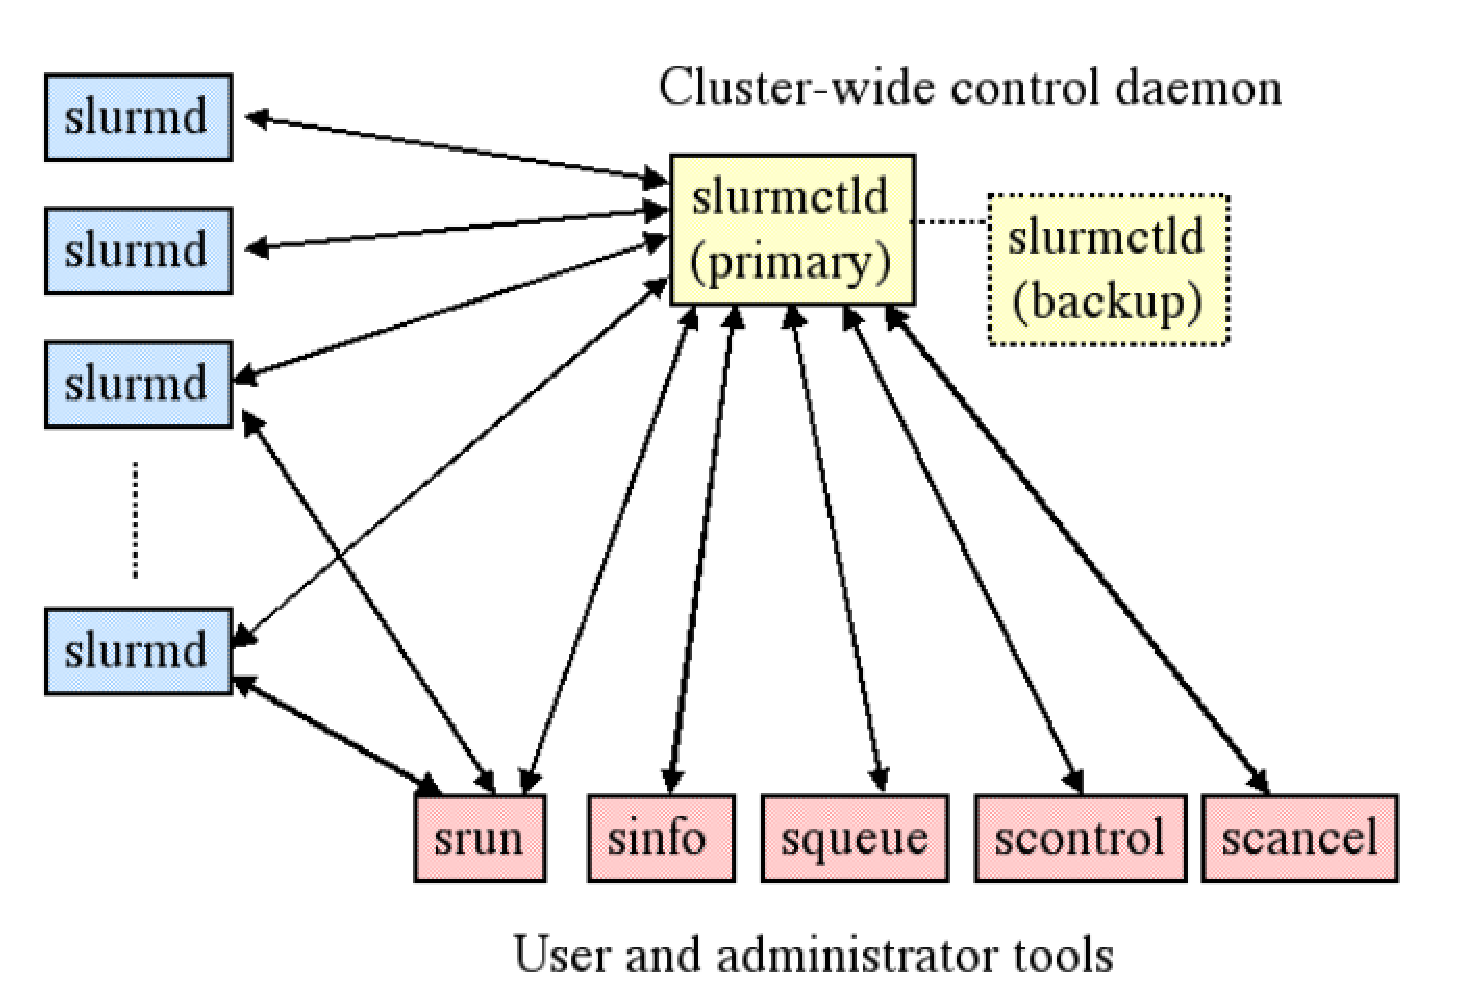
\includegraphics[height=5cm]{./images/slurm_structure.eps}}
 \caption{Slurm architecture}
\label{fig:slurm_structure}
\end{figure}

After SLURM has been installed (Sect.\ref{sec:SLURM_install}), we need to 
configure the setting on each node in the partition
(Sect.\ref{sec:SLURM-term_partition}) by creating two configuration files
\verb!slurm.conf! (required) and \verb!gres.conf! (optional) (Sect.\ref{sec:slurm_conf_file}). 

Depending on the credential authentication method we choose, we need to make
sure they have been setup propertly
\begin{itemize}
  \item OpenSSL: Sect.\ref{sec:OpenSSL}
  \item MUNGE: Sect.\ref{sec:MUNGE}. Make sure \verb!munged! daemon is started before SLURM
daemon runs (Sect.\ref{sec:MUNGE_SLURM}). 
\end{itemize}

% Before we're able to use SLURM, we need to create
% a configuration file (Sect.\ref{sec:slurm_conf_file}).

Now, we can start SLURM service
\begin{verbatim}
sudo slurmctld -D &

sudo /etc/init.d/slurm-llnl start
\end{verbatim}
To validate that SLURM is running, use \verb!sinfo! command.

BRIEF EXPLANATION: 
\begin{enumerate}
  \item  scontrol: administration tool, get/set configuration
  (Sect.\ref{sec:scontrol})
  \item  sinfo: reports general system information (Sect.\ref{sec:sinfo})
  \item  squeue: reports job and job step information - Sect.\ref{sec:SLURM-job-queue}
  \item  srun: submit/initiate job or job step (Sect.\ref{sec:srun})
  \item  scancel: signal or cancel a job or job step (Sect.\ref{sec:scancel})
\end{enumerate}


\subsection{Troubleshooting}

{\bf Troubleshooting}: Make sure a consistent version of SLURM is running on all
machines.
\begin{verbatim}
sinfo -V
rpm -qa | grep slurm
\end{verbatim}
NOTE: Version 1.1 will not work with version 1.2 or vise-versa. 
 
To check if the deamon is running
\begin{verbatim}
ps -el | grep slurmctld
\end{verbatim}

To check if the daemon (primary and backup controllers) is responding or not
\begin{verbatim}
scontrol ping
\end{verbatim}

If the daemon is running, but not responding, then
\begin{verbatim}
/etc/init.d/slurm stop
\end{verbatim}

To run/rerun the daemon with preserving the state
\begin{verbatim}
sudo /etc/init.d/slurm start
\end{verbatim}

In rare cases, if we need to restart the daemon, and losing all running jobs and
other state information, we do
\begin{verbatim}
/etc/init.d/slurm startclean
\end{verbatim}

To check why the daemon is failure, read the log file (whose name is specified
via the parameter \verb!SlurmctldLog! in the configuration file). To get more
details of log information, we increase the value of the parameter
\verb!SlurmctldDebug! in the configuration file. 

If the problem is user-specified, check if user is configured on the compute
node and management node. Make sure the UID exists on the machines. 


1. This daemon manages everything. Due to its
critical role, another node (running the backup manager) to assume the
responsibilities in the event of failure is recommended, e.g. leak.

% This tool needs a configuration file, which can be specified using either
% (following the order of descending priority)
% \begin{enumerate}
%   \item \verb!SLURM_CONF! : environment variable
%   \item run with option \verb!-f <file>!
% \end{enumerate}
% The default configuration file is \verb!slurm.conf!
% (Sect.\ref{sec:slurm_conf_file}).

% {\bf Troubleshooting}: Make sure a consistent version of SLURM is running on all
% machines.
% \begin{verbatim}
% sinfo -V
% rpm -qa | grep slurm
% \end{verbatim}
% NOTE: Version 1.1 will not work with version 1.2 or vise-versa. 
%  
% To check if the deamon is running
% \begin{verbatim}
% ps -el | grep slurmctld
% \end{verbatim}
% To check if the daemon (primary and backup controllers) is responding or not
% \begin{verbatim}
% scontrol ping
% \end{verbatim}
% If the daemon is running, but not responding, then
% \begin{verbatim}
% /etc/init.d/slurm stop
% \end{verbatim}
% To run/rerun the daemon with preserving the state
% \begin{verbatim}
% sudo /etc/init.d/slurm start
% \end{verbatim}
% In rare cases, if we need to restart the daemon, and losing all running jobs and
% other state information, we do
% \begin{verbatim}
% /etc/init.d/slurm startclean
% \end{verbatim}
% 
% To check why the daemon is failure, read the log file (whose name is specified
% via the parameter \verb!SlurmctldLog! in the configuration file). To get more
% details of log information, we increase the value of the parameter
% \verb!SlurmctldDebug! in the configuration file. 
% 
% If the problem is user-specified, check if user is configured on the compute
% node and management node. Make sure the UID exists on the machines. 


% \subsubsection{Slurmdbd}

An optional database daemon {\bf slurmdbd} to record acounting
information in a single databse. Each node has a daemon {\bf slurmld}: wait for
works, execute works, and return for more works.

% \subsection{Running a job}
% 
% Each user has a job. Once a job is assigned to a partition, the user can
% initiate parallel work in the form of {\bf job steps} in any configuration
% within the given allocation.  


\section{Inter-cluster SLURM}
\label{sec:SLURM-inter-cluster}

Slurm primarily operates on a per-cluster basis; with
\verb!slurmctld! is the 'brain' of the SLURM system for each cluster.

Example of multi-cluster system:
\begin{enumerate}
  \item  main job on one system and the "post-processing" job on the other
  (job-chaining would be useful)
  
\end{enumerate}

Efforts:
\begin{enumerate}
  \item  enhance \verb!squeue! and \verb!scontrol! to display foreign
jobs, i.e. jobs running on a different cluster.


  \item We use \verb!-M! option in sbatch (Sect.\ref{sec:sbatch}).
\url{https://slurm.schedmd.com/SUG14/inter_cluster.pdf}
  
\end{enumerate}




\section{SLURM Configuration file: slurm.conf}
\label{sec:slurm_conf_file}

SLURM need a configuration file, whose location can be specified using
either (following the order of descending priority)

\begin{enumerate}
  \item \verb!SLURM_CONF! : environment variable at runtime (or at
  compilation time using \verb!DEFAULT_SLURM_CONF! ).
    
  \item run \verb!slurmctld! with option \verb!-f <file>!.
\end{enumerate}
The default location of the configuration file is
\verb!/etc/slsurm-llnl/slurm.conf!.
Its content is described in Sect.\ref{sec:slurm.conf}.

\textcolor{red}{IMPORTANT:} This file should be consistent across all nodes in 
the cluster.

There is a tool to help generating the slurm.conf online
\footnote{\url{https://slurm.schedmd.com/configurator.html}}


\subsection{slurm.conf}
\label{sec:slurm.conf}

\textcolor{red}{NOTE: After you finish editing the configuration file,
/etc/slurm-llnl/slurm.conf, make sure to copy it to all nodes in the group of
the same security realm}.

\begin{enumerate}
  \item To generate the configuration file on SLURM 2.4 and above, use
\url{http://www.schedmd.com/slurmdocs/configurator.html}. 
  
  \item To generate the configuration file on SLURM 2.3, use
\url{https://computing.llnl.gov/linux/slurm/configurator.html}. 
   
\end{enumerate}

What we need to specify
\begin{enumerate}
  \item Control machines: the name (optinal its IP address) of the master
  machine and the backup one
  
  \item Compute machines: the names (optional their IP address) of the compute
  node; the partition name (you may have different partitions, each partition is
  a group of hosts, e.g. one for running 'debug' code, one for running 'release'
  code); the maximum running time for each job on the nodes. \textcolor{red}{No
  single node name may be listed more than once in the configuration file}.
  
Other information: number of CPUs, number of sockets, number of physical cores
per CPU, number of threads per CPU core (Sect.\ref{sec:HP_Z800})

  \item The user to run \verb!slurmctld! daemon. 
  
  \item Caching NIS information or not? (only use if slow NIS)

NOTE: If GUID caching is used (CacheGroups=1), then we need to run
\begin{verbatim}
scontrol reconfig
\end{verbatim}
everytime we made a change to system password or group databases. 
  
  \item SLURM Port number: unique port number for \verb!slurmctld! daemon to
  communicate with the \verb!slurmd! daemon on the compute nodes.
  
  \item Authentication: use MUNGE (Sect.\ref{sec:MUNGE}) is recommended. Other
  options: OpenSSL (Sect.\ref{sec:OpenSSL}).
  
  \item State Preservation: location where the state of the daemons can be saved
  (make sure we add the writing privilege to the folders for \verb!slurm! user)
  
  
  \item Scheduling: 
\begin{verbatim}
Backfill (FIFO with backfill)
Builtin (FIFO)
Gang (time-slicing for parallel jobs)
Wiki (wiki interface to meta-scheduler Maui)
Wiki2 (wiki interface to meta-scheduler Moab)
\end{verbatim}

  \item Interconnect: the SwitchType (how the nodes are connected)
  
  \item Default MPI to use: None (work with all MPIs), MPICH-GM,
MPICH-MX,  MPICH1-P4, MPICH1-SHMEM (this also works for MVAPICH-SHMEM), MPI-PMI2
(for MPI2 and MVAPICH2), MVAPICH.

  \item Process tracking: Use {\bf Pgid} (Unix Process GID)
  
  \item Resource selection
  
  \item Prolog/Epilog: the program (run by root) automatically before and after
  the user's job. The goal is to log some information if needed from that
  user's job for administration purpose.
\end{enumerate}


 A sample
\begin{verbatim}
#
# Sample /etc/slurm.conf
#
ControlMachine=cea1
ControlAddr=199.26.254.42
BackupController=cea10
BackupAddr=199.26.254.43
#
AuthType=auth/munge
Epilog=/usr/local/slurm/sbin/epilog
PluginDir=/usr/local/slurm/lib
Prolog=/usr/local/slurm/sbin/prolog
SlurmctldPort=7002
SlurmctldTimeout=120
SlurmdPort=7003
SlurmdSpoolDir=/var/tmp/slurmd.spool
SlurmdTimeout=120
StateSaveLocation=/usr/local/slurm/slurm.state
TmpFS=/tmp
#
# Node Configurations
#
NodeName=DEFAULT CPUs=4 TmpDisk=16384 State=IDLE
NodeName=lx[0001-0002] State=DRAINED
NodeName=lx[0003-8000] RealMemory=2048 Weight=2
NodeName=lx[8001-9999] RealMemory=4096 Weight=6 Feature=video
#
# Partition Configurations
#
PartitionName=DEFAULT MaxTime=30 MaxNodes=2
PartitionName=login Nodes=lx[0001-0002] State=DOWN
PartitionName=debug Nodes=lx[0003-0030] State=UP Default=YES
PartitionName=class Nodes=lx[0031-0040] AllowGroups=students
PartitionName=DEFAULT MaxTime=UNLIMITED MaxNodes=4096
PartitionName=batch Nodes=lx[0041-9999]
\end{verbatim}


To manage Nvidia GPUs, we need to add some new parameters, see
Sect.\ref{sec:SLURM_GPU}.

The configuration of each node is specified in the \verb!NodeName! line. It's
better to have each NodeName for each node, especially when the cluster is
heterogeneous. 
\begin{verbatim}
NodeName=cea22 State=UP
NodeName=cea1 State=DOWN
\end{verbatim}
If we want to put one node down, e.g. when the total memory is too low and you
don't want to schedule job on this machine, use State=DOWN. The default value
for every node can be specified in the line where NodeName=DEFAULT (there
can be multiple lines with NodeName=DEFAULT, and the value in the last line with
NodeName=DEFAULT is used). To list multiple nodes, we can use
\begin{verbatim}
NodeName=cea1,cea2,cea3
NodeName=cea[1-3]
NodeName=cea[1-3,14]
\end{verbatim}
NOTE: Up to 2 numeric ranges can be included, i.e. this is invalid
\begin{verbatim}
NodeName=cea[1-3]_linux[1-5]
\end{verbatim}
For special cases, e.g. BlueGene system, see the Manual for valid usage. 

The order of NodeName is important, as nodes will be considered adjacent in the
order they are defined.


\begin{enumerate}
  \item \url{https://computing.llnl.gov/linux/slurm/configurator.html} (SLURM
  2.3)
\end{enumerate}


\subsection{gres.conf: SLURM 2.2+}
\label{sec:gres.conf}

Generic Resource (Gres) is supported from SLURM 2.2, via a flexible plugin
mechanism. The first generic resource to be supported is GPU.
\begin{verbatim}
 ## from /etc/slurm-llnl/slurm.conf
NodeName=DEFAULT Gres=gpu:2
\end{verbatim}

\verb!/etc/slurm-llnl/gres.conf! is an ASCII file containing
information that describe generic resources being managed by SLURM on each compute
node (e.g. GPU as given in Sect.\ref{sec:SLURM_GPU}) .

Each node must have a separate \verb!gres.conf! file, if it has some generic
resource and to be scheduled by SLURM. The file represents the resource on an
individual node. The main parameter is \verb!Name=! (the name of the generic
resource which \textcolor{red}{must match the value being used for GresType
parameter in the slurm.conf}), which then accepts other parameters
\begin{itemize}
  \item \verb!File=! the full qualified pathname of the device associated with
  the resource. \textcolor{red}{IMPORTANT: Ensure the files are in increasing
  numeric order.}
  \footnote{\url{https://computing.llnl.gov/linux/slurm/gres.html}}
  
  \item \verb!Count=! the number of resources of this type (suffix can be 'K',
  'M', or 'G' which multiply 1024, 1048576 or 1073741824)

if \verb!Name=gpu!, then \verb!Count=! is not being used

if \verb!Name=gpu_mem!, then \verb!Count=! is the amount of memory in MB.

  \item \verb!CPUs=! the index of the CPUs (comma-delimited (,) or a range with
  hyphen (-)) which can use the resource. This is important on NUMA
  architecture. The starting index is zero (0). If any CPU is okay, then do not
  use this parameter to improve the speed of SLURM scheduling logic.
\end{itemize}

Example: we specify which CPU can use which GPU, which is optional. The value of
\verb!Name=! should match the value being
used for \verb!GresType=! in slurm.conf which is \verb!gpu! in this case.
\begin{verbatim}
################################################################## 
# SLURM's Generic Resource (GRES) configuration file 
################################################################## 
# Configure support for our four GPUs 
Name=gpu File=/dev/nvidia0 CPUs=0,1 
Name=gpu File=/dev/nvidia1 CPUs=0-3
Name=gpu File=/dev/nvidia2 CPUs=2,3 
Name=gpu File=/dev/nvidia3 CPUs=2,3 
Name=gpu File=/dev/nvidia4
Name=bandwidth Count=20M
\end{verbatim}

Example: We can specify which CPU to use the resource, e.g. CPU 0 uses gpu0 and
CPU 1 uses gpu1 only
\begin{verbatim}
Name=gpu File=/dev/nvidia0 CPUs=0 
Name=gpu File=/dev/nvidia1 CPUs=1 
\end{verbatim}

Example: we can specify the amount of memory in each GPU, unit of \verb!Count!
is MB if this is the same memory for all GPUs
\begin{verbatim}
Name=gpu_mem Count=2048 
\end{verbatim}

Example: we can specify the amount of memory in an individual GPU or providing
an alternative way by modifying \verb!slurm.conf! (Sect.\ref{sec:slurm_conf_file})


\subsection{Chef with SLURM}

Chef is a configuration management system.
\url{https://github.com/ajdecon/hpc-chef}

\url{http://wiki.opscode.com/display/chef/Fast+Start+Guide}

\url{http://blog.ajdecon.org/learning-chef-compute-cluster-with-slurm}

\subsection{Bright cluster management with SLURM}

\url{http://www.schedmd.com/slurmdocs/slurm_ug_2011/Bright_Computing_SLURM_integration.pdf}

\subsection{SLURM with GPUs}
\label{sec:SLURM_GPU}

From SLURM 2.2, it starts to support generic resource, first with GPU.
At first, we need a proper plugin, and modify \verb!slurm.conf!
(Sect.\ref{sec:slurm_conf_file}), as well as \verb!gres.conf!
(Sect.\ref{sec:gres.conf}. By default, a compute node has no generic resources,
i.e. no generic resources are managed by SLURM.


The parameter \verb!GresTypes! is a comma-delimited list of generic resources to
be managed by SLURM. The current support values are 'gpu' and 'nic' (network
interface card). Here we need to add 'gpu' to the list.
\begin{verbatim}
 // etc/slurm/slurm.conf
GresType=gpu
\end{verbatim}
Then, add two important parameters \verb!Feature! and \verb!Gres!, which can be
added as part of the individual \verb!NodeName! parameter to tell the
configuration for that node in a heterogeneous cluster, or at a separate lines
(which means all nodes have the same setting) for a homogeneous cluster.
\textcolor{red}{IMPORTANT: Using Gres has not been supported on IBM BlueGene
systems}.

{\bf Option one}: homogeneous cluster, i.e. all nodes have the same
configuration
\begin{enumerate}
  \item \verb!Feature! line:
  \begin{verbatim}
  Feature=''Fermi''
  \end{verbatim}

  \item \verb!Gres! contains a comma-delimited list of generic resource
  specification. Each specification consists a name, e.g. \verb!gpu!, followed
  by an optional colon (:) with a numeric value that tell how many of that
  resource.
  
Example:   A node has 2 GPUs.
  \begin{verbatim}
  Gres=gpu:2
  \end{verbatim}
\end{enumerate}

{\bf Option 2}: For a heterogeneous cluster (or even homogeneous cluster), we
can explicitly specify the configuration for individual node by adding them
as part of the parameter \verb!Nodename!.

\begin{verbatim}
NodeName=compute22 Feature=''Fermi'' Gres=gpu:1
NodeName=compute10 Feature=''Fermi'' Gres=gpu:2
\end{verbatim}
IMPORTANT: \textcolor{red}{No single node name may be listed more than once in
the configuration file}. So, we need to add after these lines.

Example: we can specify the amount of memory for an individual GPU, by adding
\verb!gpu_mem:! (unit: MB) (to specify the same memory for all GPUs, look how
we can modify gres.conf)
\begin{verbatim}
NodeName=compute22 Feature=''Fermi'' Gres=gpu:1,gpu_mem:2048
NodeName=linux[0-999] Gres=gpu:8,nic:2
\end{verbatim}

Example: we can specify the same amount of memory for all GPUs (an alternative
way is to modify gres.conf) \verb!gpu_mem! to \verb!GresType!
\begin{verbatim}
GresType=gpu,gpu_mem=2048
\end{verbatim}

NOTE: The file at all nodes must be updated properly. If all the nodes are the
same, we just modify one and distribute to all other nodes. Otherwise, we need
to modify one by one.

% We also need to create and modify the file /etc/slurm-llnl/gres.conf
% (Sect.\ref{sec:gres.conf}).


Finally, restart \verb!slurmctld!. 

\section{MPI with SLURM}

In the previous section, we introduced how to install, configure, and interact
with SLURM. A common method to run a parallel program on a cluster is using MPI.
There are different implementation of MPI protocol. We should choose one to use,
depending on the architecture of the system we have. A popular option is MPICH2.

\begin{framed}
In early version of SLURM, only Quadrics MPI uses {\bf slurmd} to initiate
tasks. Other implementations of MPI-protocol spawn processes that are not under
SLURM management. Efforts to support MPICH and LAM/MPI started in 2004. Below is
the list of MPI-implementations that have been supported.
\end{framed}

The following sections describe which MPI implementation that can be used. There
are two ways to choose which MPI implementation to use for a parallel job. 
\begin{itemize}
  \item The default MPI to be used is specified in the configuration file
  \verb!slurm.conf! via the parameter \verb!MpiDefault!. 
  
  \item Customize for a particular job with --mpi= option of the {\bf srun}
  command (or using the environment variable \verb!SLURM_MPI_TYPE!). 
\end{itemize}

SLURM supports three methods to launch parallel programs. When submiting jobs to
SLURM, depending on the MPI library being used, it can support one, two or three
methods
\begin{enumerate}
  \item Using \verb!salloc! (then use interactive SLURM shell)
  \item Using \verb!sbatch! (submit a script (noninteractive jobs) to SLURM)
  \item Using \verb!srun! (direct launching)
\end{enumerate}

OpenMPI and MPICH are both standard compliants. So, there's no difference in
programming when choosing one of them. OpenMPI comes out from MacBooks,
while MPICH is more Linux/Valgrind friendly. Also, MPICH has built-in debugger.

MVAPICH implementation support better Infiniband. Intel MPI supports
ISV\footnote{\url{http://stackoverflow.com/questions/2427399/mpich-vs-openmpi}}

\subsection{OpenMPI with SLURM}

OpenMPI supports launching parallel applications in two of the three methods
that SLURM support, with \verb!mpirun! command. The two methods are salloc and
sbatch. Then, OpenMPI will obtains the list of nodes and how many processes to
start on each node from SLURM directly.



To kill processes on different nodes, we don't need to use ssh/rsh, but use
SLURM-method (scancel). 

If the cluster is OpenFabrics network, we need to ensure SLURM set up the locked
memory properly. Otherwise, you may get error 
\begin{verbatim}
error getting openib memory
error registering openib memory of size yyyy errno says Cannot allocate memory
error creating low priority cq for mthca0 errno says Cannot allocate memory
libibverbs: Warning: RLIMIT_MEMLOCK is 32768 bytes.
error creating qp errno says Cannot allocate memory
\end{verbatim}
In some distros, the default locked memory is too low for most HPC applications.
NOTE: Ubuntu has locked memory set to ''unlimited'' already (run the command
ulimit).  To revole, either
\begin{enumerate}
  \item Edit /etc/security/limits.conf (soft)
  \begin{verbatim}
  soft memlock "unlimited"
  \end{verbatim}
  
  \item Edit  /etc/security/limits.conf (hard)
  \begin{verbatim}
  hard memlock "unlimited"
  \end{verbatim}
\end{enumerate}

Example:
\begin{verbatim}
# Allocate a SLURM job with 4 nodes
shell$ salloc -N 4 sh

# Now run an Open MPI job on all the nodes allocated by SLURM
# (Note that you need to specify -np for the 1.0 and 1.1 series;
# the -np value is inferred directly from SLURM starting with the 
# v1.2 series)
shell$ mpirun my_mpi_application


######### or
# Allocate a SLURM job with 4 nodes and run your MPI application in it
shell$ salloc -N 4 mpirun my_mpi_aplication


######### or using script
shell$ cat my_script.sh
#!/bin/sh
#!/bin/sh
#SBATCH -n 16           # 16 cores
#SBATCH -t 1-03:00:00   # 1 day and 3 hours
#SBATCH -p compute      # parition name
#SBATCH -U chemistry    # your project name - contact Ops if unsure what this is
#SBATCH -J my_job_name  # sensible name for the job
mpirun my_mpi_application

shell$ sbatch -N 4 my_script.sh
srun: jobid 1234 submitted
shell$
\end{verbatim}


\begin{enumerate}
  \item \url{http://www.open-mpi.org/faq/?category=slurm}
  \item \url{http://www.open-mpi.org/faq/?category=openfabrics#ib-locked-pages}
\end{enumerate} 

\subsection{Bluegene SLURM}

Bluegene is an IBM architecture for supercomputer targetting to
massively parallel applications. There are 3 generations: BlueGene/L,
BlueGene/P, and BlueGene/Q.

The architecture of BlueGene has many cores, Fig.\ref{fig:BlueGene_L}. The basic
block is a custom chip with two 32-bit embedded PowerPC 440 cores with custome
dual floating-point units, operating on two-element vectors. The complete
machine has 65,536 compute-nodes and 1,024 I/O nodes connecting through Gigabit
Ethernet networks. The compute nodes are partitioned and connected in a 64x32x32
three-dimensional torus network. Along with this systems, an MPI implementation,
based on MPICH2, to run on these machines with SLURM on the background is called
BlueGene MPI library. MPICH2 supports both MPI-1 and MPI-2, with optimized MPI
datatypes, optimized remote memory access (RMA), high scalability, usability and
robustness.


\begin{figure}[hbt]
  \centerline{\includegraphics[height=5cm,
    angle=0]{./images/BlueGene_L.eps}}
  \caption{BlueGene/L architecture with dual PowerPC 440 cores}
  \label{fig:BlueGene_L}
\end{figure}


\begin{enumerate}
  \item \url{https://computing.llnl.gov/linux/slurm/bluegene.html}
\end{enumerate}

\subsection{MPICH1 with SLURM}

Using MPICH1 is not recommended, please switch to using MPICH2.

\subsection{HP-MPI}

HP-MPI use \verb!mpirun! command with the -srun option to launch a job
\begin{verbatim}
$MPI_ROOT/bin/mpirun -TCP -srun -N8 ./a.out
\end{verbatim}


\subsection{MPICH2 with SLURM}

M


\subsection{MVAPICH with SLURM}

We can use the third option, i.e. srun 
\begin{verbatim}
#!/bin/sh
#SBATCH -n 16           # 16 cores
#SBATCH -t 1-03:00:00   # 1 day and 3 hours
#SBATCH -p compute      # parition name
#SBATCH -U chemistry    # your project name - contact Ops if unsure what this is
#SBATCH -J my_job_name  # sensible name for the job

srun --mpi=mvapich ./cpi.x
\end{verbatim}

\subsection{MVAPICH2 with SLURM (NVIDIA GPU)}

MVAPICH2 is based on MPICH2 and MVICH. The latest version 1.8 includes MPICH2
1.4.1p1. MVAPICH2 supports Infiniband compliant devices very good, including
high-performance communication support for nVidia GPU with IPC.

We first link mvapich2 with SLURM library
\begin{verbatim}
mpicc -L/usr/lib64 -lpmi ...
\end{verbatim}
and then we can use the third method (srun)
\begin{verbatim}
#!/bin/sh
#SBATCH -n 16           # 16 cores
#SBATCH -t 1-03:00:00   # 1 day and 3 hours
#SBATCH -p compute      # parition name
#SBATCH -U chemistry    # your project name - contact Ops if unsure what this is
#SBATCH -J my_job_name  # sensible name for the job

srun --mpi=none ./cpi.x
\end{verbatim}

\begin{enumerate}
  \item \url{http://www.tchpc.tcd.ie/node/137}
   
  \item \url{http://mvapich.cse.ohio-state.edu/overview/mvapich2/}
\end{enumerate}

\section{Termonilogies in SLURM}
\label{sec:SLURM-term_partition}
\label{sec:SLURM-term_task}

\begin{enumerate}
  \item {\bf partition}: a set of compute nodes grouped logically: shown with
  \verb!sinfo! command

The partitions can be considered job queues, each of which has an assortment of
constraints such as job size limit, job time limit, users permitted to use it, etc. 

  \item {\bf job} - Sect.\ref{sec:SLURM-job}
  
  \item {\bf a task}: is to be understood as a process.
  
NOTE: a multi-process program is made of several tasks. By contrast, a
multithreaded program is composed of only one task, which can use several CPUs. 

Tasks are requested/created with the \verb!--ntasks! option (via \verb!srun!
command - Sect.\ref{sec:SLURM-srun}), while CPUs, for the multithreaded
programs, are requested with the \verb!--cpus-per-task! option A task cannot be
split across several compute nodes, so requesting several CPUs  with the
\verb!--cpus-per-task! option will ensure all CPUs are allocated on the same
compute node.

When you run an MPI program which is expected to run with $n$ processes, SLURM
script will need to be configured to request for $n$ tasks, i.e.
\verb!--ntasks 10! if $n=10$.

Then, if the MPI program is also multi-threaded, then \verb!--cpus-per-task!
need to be configured. 

\end{enumerate}

\section{SLURM commands}

\subsection{*** arguments for any command: user, partition, state}

Many SLURM commands share common arguments, e.g. squeue
(Sect.\ref{sec:SLURM-job-queue})
\begin{verbatim}
squeue   --user <username> 
         --partition <par-name>
         --state PENDING | RUNNING | FAILED | COMPLETED
\end{verbatim}


\subsection{sinfo: information about partition}

NOTE: print node-oriented information
\begin{verbatim}
sinfo -N -l

// --format argument: 

\end{verbatim}  
NOTE: \verb!-l! just gives more information:  number of CPUs, memory, temporary
disk (also called scratch space), node weight (an internal parameter specifying
preferences in nodes for allocations when there are multiple possibilities),
features of the nodes (such as processor type for instance) and the reason, if
any, for which a node is down.  


\subsection{sstat}

It can show near-realtime information about your program (memory consumption,
etc.) with the sstat command. 
\begin{verbatim}

\end{verbatim}

\subsection{squeue: information about jobs (job queue)}
\label{sec:SLURM-job-queue}
\label{sec:squeue}

{\bf squeue}: display information about a user's job in the queue
 \begin{verbatim}
 squeue -u user1 -l
 \end{verbatim} 
with ST=status (PD=pending, R=running). 

You can filter, what user, what partition, \ldots
\begin{verbatim}
squeue   --user <username> 
         --partition <par-name>
         --state PENDING | RUNNING | FAILED | COMPLETED
\end{verbatim}

Example: output
\begin{verbatim}
JOBID PARTITION NAME USER ST  TIME  NODES NODELIST(REASON)
12345     debug job1 dave  R   0:21     4 node[9-12]
12346     debug job2 dave PD   0:00     8 (Resources)
12348     debug job3 ed   PD   0:00     4 (Priority)
\end{verbatim}
The jobid is a unique identifier that is used by many Slurm commands, e.g. if
you want to kill that job.


\subsection{-- sprio: need a plugin}

Each job is indeed assigned a priority depending on several parameter; priority
for a pending job can be obtained with \verb!sprio! command

\begin{verbatim}
tmhoangt:/home/tmhoangt/Downloads-local>sprio
You are not running a supported priority plugin
(priority/basic).
Only 'priority/multifactor' is supported.
\end{verbatim}



\subsection{scancel: cancel a job}
\label{sec:scancel}

Use jobid (provided from squeue)
\begin{verbatim}
scancel <jobid>
\end{verbatim}

\subsection{sacct}
\label{sec:sacct}

{\bf sacct}: report information about active and completed jobs
  
{\tiny
  \begin{verbatim}
sacct
  --format=jobid,jobname,account,partition,ntasks,alloccpus,elapsed,state,exitcode -j 66808
  \end{verbatim}
}

\subsection{scontrol}
\label{sec:scontrol}

{\bf scontrol}: display information about a specific job, job step, and
configuration of each node, as well as the partition
  \begin{verbatim}
#job
  
  scontrol show job
  
  scontrol show job <jobid>
  
# configuration 

  scontrol show config
    
  scontrol show partition <partitionName>
  
  scontrol show node <nodeName>
  \end{verbatim}
  or modify the attribute of a submitted job, e.g. change the partition
  \begin{verbatim}
  scontrol update jobid=$i partition=compute
  \end{verbatim}
  with \verb!$i! is the ID of the job you want to update.
 Or change all jobs on the debug partition to the compute partition.
 \begin{verbatim}
#/bin/bash
for i in $(squeue -u jtang -h -t PD -o %i)
do
scontrol update jobid=$i partition=compute
done
 \end{verbatim}

\subsection{sinfo}
\label{sec:sinfo}

 {\bf sinfo}: display states and partition name of each node 

{\tiny
\begin{verbatim}
$>sinfo

PARTITION AVAIL  TIMELIMIT  NODES  STATE MIDPLANELIST
main*        up 30-00:00:0   2632  alloc bgq[0001x1011,0010x1010,1000]
main*        up 30-00:00:0   1464   idle bgq[0000x1010,0011x1011,1001]
testing      up      15:00    381  alloc bgq1011
testing      up      15:00    131   idle bgq1011
filler       up 30-00:00:0   2632  alloc bgq[0001x1011,0010x1010,1000]
filler       up 30-00:00:0   1464   idle bgq[0000x1010,0011x1011,1001]


Asterisk(*) in PARTITION = default partition. Timelimit=days:hours:mins:secs.
Asterisk(*) in STATE  = it's not responding.

\end{verbatim}
}
  
  \begin{verbatim}
  
  # partition named 'debug'
  sinfo -p debug
  \end{verbatim}
  {\bf sinfo} will display  lists of partitions you are allowed to use. To list
  all, use sinfo -a.
 
\subsection{smap}
\label{sec:smap}

{\bf smap}: display graphical information about jobs and partitions
\begin{verbatim}
smap -i 2
\end{verbatim}

Press 'q' to quit.

\section{Submit a job}
\label{sec:SLURM-job}

You can submit a job using either
\begin{enumerate}
  \item \verb!salloc! (allocate resources) + \verb!srun! (launch the job) 
  
  \item \verb!sbatch! (which requires a script file -
  Sect.\ref{sec:SLURM-submission-script} - that describes both resources
  required and the command at the end to launch the job) - Sect.\ref{sec:sbatch}  
\end{enumerate}


{\bf a job}: A job consists in two parts:
  \begin{itemize}
    \item {\bf resource request}:
   Resource requests consist in a number of CPUs, computing expected
  duration, amounts of RAM or disk space, etc. 
   
    \item {\bf job step}: A job step describe a sets of (possibly parallel)
    tasks within a job.
      
 NOTE: The SLURM script (as being described below) is itself a job step. 
 Other job steps are created with the \verb!srun! command.
 
  \end{itemize}

Priority-ordered jobs are allocated nodes within a partition until the resources
(nodes, processors, memory, etc.) within that partition are exhausted.


At the end of the script describe a program to run.

A {\bf task} is described in
Sect.\ref{sec:SLURM-term_task}.

\subsection{srun}
\label{sec:SLURM-srun}
\label{sec:srun}

You can launch the simulation with \verb!srun! as a shell command; after the
resource has been requested using \verb!salloc! command
(Sect.\ref{sec:SLURM-salloc}); or \verb!srun! can also be used within
\verb!sbatch!'s script-file or \verb!salloc!'s input.

WARNING:  When  srun  is  executed from within salloc or sbatch, there are
configurations and options which can result in  inconsistent  allocations when
\verb!-c! of srun has a value greater than -c on salloc or sbatch.


There are many options you can pass with \verb!srun! 
\footnote{\url{https://computing.llnl.gov/tutorials/moab/man/srun.txt}}
but here is a few
\begin{enumerate}
  
  \item The -n, -c, and -N options control how CPUs  and nodes  will  be  allo-
       cated  to  the job.
  \begin{itemize}
    \item Only \verb!-n! (number of processes to run)
    it assumes 1 CPU per processes is allocated.
    
    So, this by default is not allowed to exceed the total number of CPUs 
    
    \item When \verb!-c! is also used (it controls number of CPU per
    process/task)
    
    
    \item When \verb!-N! is also used (it controls number of nodes to be
    allocated)
  \end{itemize}     
       
  \item \verb!--cores-per-socket! = 
  restrict to using nodes with at least the specified number of cores per socket
  
  NOTE: This is needed with task/affinity plugin is enabled.
  It may needs \verb!-B! option.
  
  \item \verb!--cpu_bind=! [quiet, verbose]
  
  NOTE: This is needed when task/affinity plugin is enabled.
  
  \item \verb!-c! (or \verb!--cpus-per-task!): default is 1 CPU per task.
  (request ncpus be allocated per process.)
  
  This may be useful if the job is multithreaded and requires more than one  CPU
   per task  for  optimal  performance.
              
  \item 
  
\end{enumerate}


\subsection{salloc}
\label{sec:SLURM-salloc}


\subsection{sinteractive}
\label{sec:sinteractive}

Interactive sessions allow you to connect to a compute node and work on that
node directly. This allows you to develop how your jobs might run (i.e. test
that commands run as expected before putting them in a script) and do heavy
development tasks that cannot be done on the login nodes (i.e. use many cores)

\begin{verbatim}
sinteractive --mem=Mg --cpus-per-task=C 	interactive job with 4 CPUs and M GB of
memory on a shared node.
\end{verbatim}

\url{https://www.massive.org.au/userguide/running-slurm-jobs/running-interactive-jobs}

\subsection{sbatch}
\label{sec:sbatch}

In addition to the setting defined in the script, we can also pass options to
sbatch
\begin{verbatim}
sbatch [options] <script-file-name>
\end{verbatim}

NOTE:
\begin{enumerate}
  \item  The script-file-name's content is described in
Sect.\ref{sec:SLURM-submission-script}.

  \item options:
  
  
\begin{itemize}
  \item \verb!--mem=8g!  : request 8GB on a shared node
  
  \item \verb!--mem=8g --cpus-per-task=4! : request 8GB on a shared node, and 4
  CPUs
  
\end{itemize}   
\end{enumerate}

sbatch exits immediately after the script is  successfully  transferred to  the
SLURM controller and assigned a SLURM job ID.
\begin{enumerate}
  \item as the script also request resources
  
  If requested resources are not available, the job is in the queue
  (Sect.\ref{sec:SLURM-job-queue}). Once the resources is approved and reserved
  for the job, a \textcolor{red}{job allocation number} is also generated.
  
  \item both standard output/input are directed to a file:
  \verb!slurm-%j.out! (with \verb!%j! is replaced with job allocation number)
  
 File is stored on the first node of the job allocation.
 

  \item with the {\bf job allocation number}:
  \begin{enumerate}
    \item 
  SLURM only copy the script to the first node in the allocated resources (BUT
  NO any other user's fifles; so it is expected a shared mounted home directory
  is available across the nodes)
  
    \item SLURM run a \textcolor{red}{single copy of the batch script} on the
    first node (in the set of allocated nodes)
   
    
  \end{enumerate}
  
  
\end{enumerate}





\section{submission script}
\label{sec:SLURM-submission-script}

To submit a job, we write a submission script, e.g. \verb!slurm.sh!, which is a
shell (e.g. bash) script, 
\begin{enumerate}
  \item first line: describe the shell environment
  
  \item a series of \verb!#SBATCH! statements
  
NOTE: sbatch  will stop  processing  options  at  the first line which does NOT begin
with  \verb!"#SBATCH"!.
  
  \item executable command line: the command to launch the parallel program 
\end{enumerate}


SLURM will extract comments (starting with
\verb!#!), prefix with \verb!SBATCH!, as parameters describing {\it resource
requests}. 

\begin{mdframed}
If you are an admin: make sure SLURM is installed and configured properly on
every machine in the partition (Sect.\ref{sec:SLURM}). 
\end{mdframed}

To launch the script, run with \verb!sbatch! command (Sect.\ref{sec:sbatch}).

Helps:
\begin{itemize}
  \item    \url{https://ubccr.freshdesk.com/support/solutions/articles/5000688140-submitting-a-slurm-job-script}
  
\end{itemize}

%\section{Running jobs with SLURM}


% Now to run the MPI job on the partition, (1) create an executable script (which
% include a list of SLURM directives or commands to tell the job scheduler what
% to do) , (2) run the script with a SLURM command, e.g.
% \verb!sbatch!.
% \begin{enumerate}
%   \item syntax for the SLURM directive in a script:
%   
%   \verb!#SBATCH <flag>!
%   
% \end{enumerate}
\subsection{-- chose the partition}

\subsection{-- choose the resource using time}

\subsection{--- choose number of nodes/what nodes in that partition}

\subsection{-- for single-processor apps}

\begin{verbatim}
#SBATCH --ntasks=1                    # Run on a single CPU
#SBATCH --ntasks=1   
# Run on a single CPU #SBATCH --mem=600mb                   # Memory limit

# your code here
pwd; hostname; date
module load python
echo "Running plot script on a single CPU core"
python /ufrc/data/training/SLURM/plot_template.py
date
\end{verbatim}

\subsection{-- for threadaed or multi-processor job}

Apps (OpenMP, PTHREADS, or shared memory applications) using multiple processors
on a single server. While they can use multiple processors, they cannot make use
of multiple servers and all the processors must be on the same node.

\begin{verbatim}
# must set
##SBATCH --nodes=1
# must set to the number of OpenMP threads you wish to use
##SBATCH --cpus-per-task

#SBATCH --nodes=1                    # Use one node
#SBATCH --ntasks=1                   # Run a single task	
#SBATCH --cpus-per-task=4            # Number of CPU cores per task
#SBATCH --mem=600mb                  # Total memory limit

# run the app (and tell it how many processors to use)
# this depends on app, e.g. option to
# set OMP_NUM_THREADS or use command-line option when calling the app
pwd; hostname; date
 
echo "Running prime number generator program on $SLURM_CPUS_ON_NODE CPU cores"
 
module load gcc/5.2.0 
/ufrc/data/training/SLURM/prime/prime
date
\end{verbatim}

\begin{verbatim}
#!/bin/sh
#SBATCH --job-name=parallel_job_test # Job name
#SBATCH --mail-type=ALL              # Mail events (NONE, BEGIN, END, FAIL, ALL)
#SBATCH --mail-user=<email_address>  # Where to send mail	
#SBATCH --nodes=1                    # Use one node
#SBATCH --ntasks=1                   # Run a single task	
#SBATCH --cpus-per-task=4            # Number of CPU cores per task
#SBATCH --mem=600mb                  # Total memory limit
#SBATCH --time=00:05:00              # Time limit hrs:min:sec
#SBATCH --output=parallel_%j.out     # Standard output and error log
 
export OMP_NUM_THREADS=4
module load intel
./YOURPROGRAM INPUT
\end{verbatim}

\subsection{-- MPI app}

 These are applications that can use multiple processors that may, or may not,
be on multiple servers.

\subsection{-- example 1}

\textcolor{red}{Step 1}: write the script
\begin{verbatim}
#!/bin/bash
#### the configuration when launching the job
# always start with #SBATCH

# choose partition 'debug'
#SBATCH -p debug
 
# request how many nodes?
# use this #SBATCH -n 1
# or this #SBATCH --nodes=1

# request run-time 
#SBATCH -t 12:00:00

# define job name
# use this #SBATCH -J some_job_name
# or  this #SBATCH --job-name="FastMag_Test_1"

#SBATCH --ntasks=1
#SBATCH --cpus-per-task=1
#SBATCH --ntasks-per-node=1

###
### the real job run on each node  
ls / > /home/vagrant/slurm.out
\end{verbatim}

The real job sent to the cluster (partition) can be a simple Linux command, a
shell sript file, or an executable file.

The list of all commands: \verb!sacct!, \verb!salloc!, \verb!sattach!,
\verb!sbatch!, \verb!sbcast!, \verb!scancel!, \verb!scontrol!, \verb!sinfo!,
\verb!smap!, \verb!squeue!,  \verb!srun!, \verb!strigger! and \verb!sview!.
User tools: {\bf srun} to initate the job, {\bf scancel} to cancel a queuing or
terminate a running job, {\bf sinfo} to report system status, {\bf squeue} to
report the status of jobs, {\bf sacct} to get information about jobs (running
or have completed). We can also use {\bf smap, sview} for graphical report of
jobs, including network topology. Since SLURM 2.4: {\bf sdiag} repots scheduling
statistics. 

For administrator: {\bf scontrol} to monitor and/or modify configuration and
state information on the cluster, {\bf sacctmgr} to manage database. 

\subsection{Using GPU}

First, the generic resource GPU need to be configured on each node
(Sect.\ref{sec:SLURM_GPU}). Then, we launch a simulation and specify the GPU as
the generic resource to use via \verb!--gres=gpu! option to the commands
\verb!srun, sbatch!, or \verb!salloc!. The syntax is
\begin{verbatim}
--gres=name[:count]
\end{verbatim}

Example: to use GPU we add \verb!--gres=gpu! to the
batch command line
\begin{verbatim}
sbatch -N 2 -n 4 --gres=gpu

sbatch -N 2 -n 4 --gres=gpu:1

sbatch -N 2 -n 4 --gres=gpu:2
\end{verbatim}

Example: to limit which GPU to use with \verb!--constraint=! option
\begin{verbatim}
 // any Fermi-based GPU card
sbatch -N 2 -n 4 --gres=gpu:1 --constraint="Fermi"

 // Fermi-based Gefore card only
sbatch -N 2 -n 4 --gres=gpu:1 --constraint="Fermi|geforce"
\end{verbatim} 

Example: select node based upon GPU memory (unit: MB), add \verb!,gpu_mem=!
after \verb!--gres=!, e.g. at least 2000 MB. REQUIREMENT: \textcolor{red}{We
must specify how much memory for each GPU at the gres.conf file}
(Sect.\ref{sec:gres.conf})
\begin{verbatim}
sbatch -N 2 -n 4 --gres=gpu,gpu_mem:2000 
\end{verbatim} 

References:
\begin{enumerate}
  \item
  \url{http://www.hpc-ch.org/wp/wp-content/uploads/2011/11/CSCS_Schedule_GRES_with_SLURM.pdf}
\end{enumerate}


\subsection{Launch Commands}

There are two ways to launch a parallel jobs using SLURM:
\begin{enumerate}
  \item You can call \verb!salloc! to allocate the resource, and then use
  \verb!srun! to run the parallel program. NOTE: \verb!srun! can do the job of
  \verb!salloc! too, so we just need \verb!srun! only.
  
  \item Using a script which contains a number of command: we use \verb!sbatch!
  to run the script.
  \begin{verbatim}
  sbatch slurm_SCRIPTNAME
  \end{verbatim}
\end{enumerate}

DETAILED EXPLANATION: A list of commands to control both the compute node and
the management node is: 
\begin{enumerate}
  \item {\bf salloc}: allocate resources for jobs, and spawn a shell, from which
  we can use {\bf srun} to launch one or more parallel jobs. It's possible to
  allocate resource and run the parallel job using a single {\bf srun} command. 
  \begin{verbatim}
  srun -n4 -N3 -l /bin/myprogram 
  \end{verbatim}
  Here, we execute 4 tasks (-n4) of /bin/myprogram on three nodes (-N3), and
  include task number on the output. The default partition is used, with one task per node per
  processor.
  \begin{verbatim}
  #run 4 tasks on a single (current) node 
    srun -n4 -l /bin/myprogram  
  \end{verbatim}
  
  For more detail control, read {\bf srun} command. A common mode of operation
  is to submit a script for later execution (see sbatch). 

  \item {\bf srun}: with 13 different command-line options, it can (1) run job,
  (2) allocate resources, (3) submit patch jobs, (4) attach to a currently
  running job, (5) launch job step (a set of parallel tasks).
   \begin{itemize}
     \item \verb!--ntasks=4! : create 4 tasks (and implicitly use 4 processors)
     resource allocation (job) in a given partition
     \item \verb!--node=min-max! : explicitly tell node count between [min,max]
     \item \verb!--node=4! : explicitly tell node count minimum is 4
     \item \verb!--partition=pdebug! : select the partition
     \item \verb!--label! : labeling the output
     \item \verb!--attach=<jobID>!: attach in read-only mode, i.e. standard
     error and output from job <jobID> are sent to this srun, along with any
     pre-existing srun command that associte with job <jobID>.
     \item \verb!--attach=<jobID> --join!: attach current srun to the job
     <jobID> and also allow standard input and signals from this srun to be
     forwarded to the job <jobID>.
     
     \item \verb!/bin/your_mpi_job! : a program you want to run
   \end{itemize}
   Example: simply print out the host name of the 4 machines in the partition
   name \verb!pdebug!
   \begin{verbatim}
   srun --ntasks=4 --partition=pdebug --label /bin/hostname
   srun -n 4 -p pdebug -l /bin/hostname
   \end{verbatim}
     
  \item {\bf sattach}: attach/detach (one or multiple times) a standard
  input/output/error plus signal capabilities to a running parallel job.
  
  \item {\bf sbatch}: submit a job script (which contains one or more {\bf
  srun} commands and \verb!#SBATCH! configuration) for using multiple
  times.  Suppose the script is
  \begin{verbatim}
#!/bin/bash
sbcast my.prog /tmp/my.prog
srun /tmp/my.prog

## or
mpirun /tmp/my.prog 
  \end{verbatim}
then we run
\begin{verbatim}
### run on 8 nodes
$home> sbatch --nodes=8 my.job
srun: jobid 12345 submitted

### or specify the partition (and 10 processes)
$home> sbatch -p PARTITION_NAME -n 10 my.job

### to use Infiniband
$home> sbatch -p PARTITION_NAME -C infiniband -n 10 jobscript.sh
\end{verbatim}  


  \item {\bf sbcast}: transfer a file to a local disk on ALL nodes
  allocated for the job (e.g. the parallel binary excutable file). This should
  be used within a batch job or within a shell spawn after calling {\it salloc}. 
  \begin{verbatim}
  sbcast [-CfpstvV] SOURCE DEST
  \end{verbatim}
  SOURCE = name of file on current node; DEST = full qualified path name (to be
  copied on each node) and should be local disk (not the shared file system). 
  NOTE: -C = compress the file, -f = force (replace existing destination), -p =
  preseve datetime/mode/access of the file.
    
  \item {\bf scancel}: cancel a pending or running job/job step (by sending
  SIGKILL signal); or send an arbitrary signal to all processes associated with
  a running job/job step.
  \begin{verbatim}
  scancel <jobID>
  scancel --user=<userID>  // cancel all 
  scancel --interactive --user=<userID>   //cancel with questions
  \end{verbatim}
\end{enumerate}

\subsection{Cancel a job}

Check the JOB ID with 
\begin{verbatim}
squeue
\end{verbatim}

and then issue 
\begin{verbatim}
scancel <JOBID>
\end{verbatim}

\subsection{Setting job priority (reservation)}

Sometimes, you want to set one simulation to get a higher priority to run first,
or you want to reserve a number of nodes at a certain time preriod so that no
other jobs can use these resources. That can be done with specifying these in
the batch file

\begin{verbatim}
#SLURM reservation=CARDIOID-20130404
#SLURM queue=reserved
\end{verbatim}
with \verb!CARDIOID-20130404! is the name that you create.

\subsection{Why my task is}

Jobs are run based on First-in-First-out scheduling. However, Jobs can get held
(prioprity = 0) if it exceeds the partition constraints, e.g. node count too,
time limit, etc.

\subsection{Log file}

To check why a block is in error state, grep for \verb!update_block! in the
configuration file.

After fixing the problem, we need to manually fix the block
\begin{verbatim}
sfree -b BLOCKNAME

# to run all the blocks
sfree -a
\end{verbatim}
or using scontrol
\begin{verbatim}
scontrol update state=FREE BlockName=BLOCKNAME
\end{verbatim}

\chapter{TORQUE/Maui; TORQUE/Moab}
\label{chap:TORQUE}

TORQUE is a very popular batch system usually deployed in conjunction with the
Maui scheduler. TORQUE is a community effort based on PBS

It also very popular across small and medium clusters and it is the main batch
system.

\chapter{PBS}
\label{chap:PBS}


\section{PBS convert to SLURM}
\label{sec:PBS-convert-SLURM-script}

\url{https://hpc.nih.gov/docs/pbs2slurm.html}


\chapter{Sun Grid Engine (SGE)}
\label{chap:SGE}
\label{sec:OGS}
\label{sec:SoG}

Sun Grid Engine (SGE) is one of many batch systems, along with SLURM
(Sect.\ref{sec:SLURM}) and TORQUE/Maui (Sect.\ref{chap:TORQUE}).

The acquisition of Sun by Oracle has ended the Grid Engine open-source project
but two alternative forks have appeared: Open Grid Scheduler (OGS) and Son of
Grid Engine (SoG). Of the two the only one that can be really considered under
active development is SoG with 4 new releases in 2013. The OGS variant has not
received any update since May 8, 2012.
